% \begin{name}
% 	{GV biên soạn: Nguyễn Hữu Trung Kiên\\ GV phản biện: Phúc Hậu}
% 	{TOÁN 10-KNTT-CS}
% \end{name}
\newpage
\setcounter{section}{10}
\section{Tích vô hướng của hai vectơ}
\subsection{KIẾN THỨC TRỌNG TÂM}
\subsubsection{Góc giữa hai vectơ}
\begin{khung4}{}
\immini{Cho hai vectơ $\vec{a}$ và $\vec{b}$ đều khác $\vec{0}$. Từ một điểm $O$ bất kì ta vẽ $\vec{OA}=\vec{a}$, $\vec{OB}=\vec{b}$.\begin{itemize}
\item Góc $\widehat{AOB}$ với số đo từ $0^\circ$ đến $180^\circ$ được gọi là \textbf{góc giữa hai vectơ} $\vec{a}$ và $\vec{b}$.
\item Ta kí hiệu góc giữa hai vectơ $\vec{a}$ và $\vec{b}$ là $\left(\vec{a},\vec{b}\right)$.
\item Nếu $\left(\vec{a},\vec{b}\right)=90^\circ$ thì ta nói rằng $\vec{a}$ và $\vec{b}$ vuông góc với nhau, kí hiệu là $\vec{a}\perp \vec{b}$.
\end{itemize}
}
{
\begin{tikzpicture}[scale=1.5, font=\footnotesize, line join=round, line cap=round, >=stealth]
	\path
	(-3,0) coordinate (O)
	(O)+(30:1) coordinate (A)
	(O)+(-45:2) coordinate (B)
	;
	\draw[->] (O)++(-2,1)--+(-45:2) node[above,pos=0.5,sloped] {$\vec{b}$};
	\draw[->] (O)++(-2,-1)--+(30:1) node[below,pos=0.5,sloped] {$\vec{a}$};
	\draw[->] (O)--(A) node[above,pos=0.5,sloped] {$\vec{a}$};
	\draw[->] (O)--(B) node[above,pos=0.5,sloped] {$\vec{b}$};
	\foreach \p/\r in {O/180,A/90,B/-90}
	\fill (\p) circle (1pt) node[shift={(\r:3mm)}]{$\p$};
\end{tikzpicture}
}\end{khung4}
\begin{khung4}{}\,
\begin{itemize}
		\item Từ định nghĩa, ta có $\left(\vec{a},\vec{b}\right)=\left(\vec{b},\vec{a}\right)$.
		\item Góc giữ hai vectơ cùng hướng và khác $\vec{0}$ luôn bằng $0^\circ$.
		\item Góc giữa hai vectơ ngược hướng và khác $\vec{0}$ luôn bằng $180^\circ$.
		\item Trong trường hợp có ít nhất một trong hai vectơ $\vec{a}$ hoặc $\vec{b}$ là vectơ $\vec{0}$ thì ta quy ước số đo góc giữa hai vectơ đó là tùy ý (từ $0^\circ$ đến $180^\circ$).
	\end{itemize}
\begin{center}
	\begin{tikzpicture}[scale=1, font=\footnotesize, line join=round, line cap=round, >=stealth]
		\begin{scope}
			\path
			(0,0) coordinate (O)
			;
			\draw[->,line width=1pt] (O)--+(0:1) node[above,sloped,pos=.5]{$\vec{a}$};
			\draw[->] (O)--+(0:2) node[above,sloped,pos=.8]{$\vec{b}$};
			\draw[fill=black] (O) circle (1pt);
			\node at ($(O)+(1,-.5)$) {$\left(\vec{a},\vec{b}\right)=0^\circ$};
		\end{scope}
		\begin{scope}[xshift=6cm]
			\path
			(0,0) coordinate (O)
			;
			\draw[->,line width=1pt] (O)--+(0:1) node[above,sloped,pos=.5]{$\vec{d}$};
			\draw[->] (O)--+(180:2) node[above,sloped,pos=.8]{$\vec{c}$};
			\draw[fill=black] (O) circle (1pt);
			\node at ($(O)+(-.5,-.5)$) {$\left(\vec{c},\vec{d}\right)=180^\circ$};
		\end{scope}
	\end{tikzpicture}
\end{center}
\end{khung4}
\subsubsection{Tích vô hướng của hai vectơ}
\begin{khung4}{}
	Cho hai vectơ $\vec{a}$ và $\vec{b}$ đều khác $\vec{0}$.\\
	\textbf{Tích vô hướng} của $\vec{a}$ và $\vec{b}$ là một số, kí hiệu là $\vec{a}\cdot \vec{b}$, được xác định bởi công thức
	$$\vec{a}\cdot \vec{b}=\left|\vec{a}\right|\cdot \left |\vec{b}\right|\cdot \cos \left(\vec{a},\vec{b}\right).$$
\end{khung4}
\begin{khung4}{}\,
	\begin{itemize}
		\item Trường hợp ít nhất một trong hai vectơ $\vec{a}$ và $\vec{b}$ bằng $\vec{0}$, ta quy ước $\vec{a}\cdot \vec{b}=0$.
		\item Với hai vectơ $\vec{a}$ và $\vec{b}$, ta có $\vec{a}\perp \vec{b}\Leftrightarrow \vec{a}\cdot \vec{b}=0$.
		\item Khi $\vec{a}=\vec{b}$ thì tích vô hướng $\vec{a}\cdot \vec{b}$ được kí hiệu là $\vec{a}^2$ và được gọi là \textit{bình phương vô hướng} của vectơ $\vec{a}$.\\
		Ta có $\vec{a}^2=\left|\vec{a}\right|\cdot \left|\vec{a}\right|\cdot \cos 0^\circ=\left|\vec{a}\right|^2$. Vậy bình phương vô hướng của một vectơ luôn bằng bình phương độ dài của vectơ đó.
	\end{itemize}
\end{khung4}
\subsubsection{Biểu thức tọa độ và tính chất của tích vô hướng}
\begin{tc}
	Cho $\vec{a}=(x;y)$, $\vec{b}=(x';y')$, ta có
	$$\vec{a}\cdot \vec{b}=x\cdot x'+y\cdot y'.$$
\end{tc}
\begin{tc}
	Với ba vectơ $\vec{a}$, $\vec{b}$, $\vec{c}$ bất kì và mọi số thực $k$, ta có
	$$\vec{a}\cdot \vec{b}=\vec{b}\cdot \vec{a};\qquad \vec{a}\cdot \left(\vec{b}+\vec{c}\right)=\vec{a}\cdot \vec{b}+\vec{a}\cdot \vec{c};\qquad \left(k\vec{a}\right)\cdot \vec{b}=k\left(\vec{a}\cdot \vec{b}\right)=\vec{a}\cdot \left(k\vec{b}\right).$$
\end{tc}
\subsection{PHÂN LOẠI VÀ PHƯƠNG PHÁP GIẢI TOÁN}
\begin{dang}{Tính tích vô hướng hoặc dùng bình phương vô hướng để tính độ dài}
	Đưa hai vectơ về cùng gốc và sử dụng công thức:
$$\overrightarrow{AB}\cdot \overrightarrow{AC}=AB\cdot AC\cdot \cos \widehat{A}.$$
\begin{itemize}
        \item Diện tích tam giác đều $ S_{\triangle \text{đều}}=\dfrac{(\text{cạnh})^2\times\sqrt{3}}{4} $, suy ra chiều cao tam giác đều $ =\dfrac{\text{cạnh}\times\sqrt{3}}{2} $.
        \item Diện tích hình vuông $ S_\text{Hình vuông}=(\text{cạnh})^2 $, suy ra đường chéo hình vuông $ =\text{cạnh}\times \sqrt{2} $.
    \end{itemize}
    \end{dang}
\begin{vd}%[0H5H4-1]%[Biên soạn tài liệu dạy học bộ KNTT - CS]%[GVBS Nguyễn Hữu Chung Kiên]
	Cho hình vuông $ABCD$ cạnh bằng $2a\sqrt{2}$. Tính tích vô hướng $\overrightarrow{AB}\cdot \overrightarrow{AC}.$
\loigiai{
	\immini{Ta có $\overrightarrow{AB}.\overrightarrow{AC}=\left|\overrightarrow{AB}\right|\cdot \left|\overrightarrow{AC}\right|\cdot \cos\left(\overrightarrow{AB},\overrightarrow{AC}\right).$
	\\Vì tam giác $ABC$ vuông tại $B$ nên $$AC^2=AB^2+BC^2=\left(2a\sqrt{2}\right)^2+\left(2a\sqrt{2}\right)^2=16a^2\Rightarrow AC=4a.$$ Suy ra $\overrightarrow{AB}\cdot \overrightarrow{AC}=2a\sqrt{2}\cdot 4a\cdot \cos 45^\circ=8a^2.$}{
	\begin{tikzpicture}[scale=.7,>=stealth]
		\coordinate [label=left:$A$](A) at (0,6);
		\coordinate [label=below:$B$](B) at (0,0);
		\coordinate [label=below:$C$](C) at (6,0);
		\coordinate[label=right:$D$] (D) at ($(C)-(B)+(A)$);
		\foreach \x/\y/\z in {A/B/C}{\draw pic[draw,angle radius=2mm]{right angle=\x--\y--\z};}
		\foreach \diem in {A,B,C,D}	\fill (\diem)circle(1pt);
		\draw[smooth](A)--(D)--(C)--(B);
		\draw[->](A)--(B);
		\draw[->](A)--(C);
	\end{tikzpicture}}
	}
\end{vd}
\begin{vd}%[0H5V4-1]%[Biên soạn tài liệu dạy học bộ KNTT - CS]%[GVBS Nguyễn Hữu Chung Kiên]
	Cho tam giác $ABC$ đều cạnh $a$, tâm $O$. Hãy tính
	\begin{enumEX}[a)]{2}
		\item $\vec{AB} \cdot \vec{AC}$.
		\item $\vec{AB} \cdot \vec{BC}$.
		\item $\left(\vec{OB}+\vec{OC}\right)\cdot \left(\vec{AB}-\vec{AC}\right)$.
		\item $\left(\vec{AB}+2\vec{AC}\right)\cdot \left(\vec{AB}-3\vec{BC}\right)$.
	\end{enumEX}
\loigiai{
	\begin{center}
		\begin{tikzpicture}[line join=round, line cap=round,scale=.7]
			\def\canh{5}
			\coordinate (B) at (0,0);
			\coordinate (C) at (\canh,0);
			\coordinate (A) at ($(B) + (60:\canh)$);
			\coordinate (D) at ($(A) + (\canh,0)$);
			\path (A)--(B) node[midway,sloped,scale=0.5]{$|$};
			\path (A)--(C) node[midway,sloped,scale=0.5]{$|$};
			\path (B)--(C) node[midway,sloped,scale=0.5]{$|$};
			\coordinate (Tempta) at ($(A)!0.5!(B)$);
			\coordinate (Temptb) at ($(A)!0.5!(C)$);
			\coordinate (Temptc) at ($(Tempta)!1cm!90:(A)$);
			\coordinate (Temptd) at ($(Temptb)!1cm!90:(A)$);
			\coordinate (O) at (intersection of Tempta--Temptc and Temptb--Temptd);
			\coordinate (I) at ($(B)!0.5!(C)$);
			\coordinate (E) at ($(O)!2!(I)$);
			\draw(A)--(B)--(C)--cycle (E)--(B)--(O)--(C) (O)--(E) (A)--(D);
			\foreach \i/\g in {A/90,B/-90,C/-90,O/90,E/-90,D/90}{\draw[fill=black](\i) circle (1.5pt) ($(\i)+(\g:3mm)$) node[scale=1]{$\i$};}
		\end{tikzpicture}
	\end{center}
	\begin{enumerate}
		\item Tam giác $ABC$ đều, suy ra $\widehat{BAC}=60^{\circ}$.\\
		Theo định nghĩa
		\begin{center}
			$\vec{AB} \cdot \vec{AC}=\left|\vec{AB}\right|\cdot\left|\vec{AC}\right|\cos\left(\vec{AB},\vec{AC}\right)=\left|\vec{AB}\right|\cdot\left|\vec{AC}\right|\cos\widehat{BAC}=a\cdot a \cdot \cos 60^{\circ}=\dfrac{a^2}{2}$.
		\end{center}
		\item Gọi $D$ là điểm sao cho $\vec{AD}=\vec{BC}$.\\
		Vì $AD\parallel BC$ nên $\widehat{DAC}=\widehat{ACB}=60^{\circ}$.\\
		Suy ra $\widehat{BAD}=\widehat{DAC}+\widehat{BAC}=60^{\circ}+60^{\circ}=120^{\circ}$.
		\begin{center}
			$\vec{AB} \cdot \vec{BC}=\vec{AB} \cdot \vec{AD}=\left|\vec{AB}\right|\cdot\left|\vec{AD}\right|\cos\left(\vec{AB},\vec{AD}\right)=\left|\vec{AB}\right|\cdot\left|\vec{AD}\right|\cos\widehat{BAD}=a\cdot a \cdot \cos 120^{\circ}=-\dfrac{a^2}{2}$.
		\end{center}
		\item Gọi $E$ là điểm sao cho $\vec{BE}=\vec{OC}$.\\
		Ta có $\vec{OB}+\vec{OC}=\vec{OB}+\vec{BE}=\vec{OE}$; $\vec{AB}-\vec{AC}=\vec{CB}$.\\
		Do đó $\left(\vec{OB}+\vec{OC}\right)\cdot \left(\vec{AB}-\vec{AC}\right)=\vec{OE}\cdot \vec{CB}$.\\
		Vì $OC\parallel BE$ và $OC=BE$ nên tứ giác $OBEC$ là hình bình hành.\\
		$O$ là trọng tâm tam giác $ABC$, suy ra $OB=OC$.\\
		Hình bình hành $OBEC$ có $OB=OC$ nên là hình thoi.\\
		Suy ra $OE\perp BC$.\\
		Suy ra $\vec{OE}\cdot \vec{CB}=0$ (hai đường chéo hình thoi).\\
		Vậy $\left(\vec{OB}+\vec{OC}\right)\cdot \left(\vec{AB}-\vec{AC}\right)=0$.
		\item Ta có
		$\vec{AC}\cdot\vec{BC}=\left|\vec{AC}\right|\cdot\left|\vec{BC}\right|\cos\left(\vec{AC},\vec{BC}\right)=\left|\vec{AC}\right|\cdot\left|\vec{BC}\right|\cos\widehat{ACB}=a\cdot a\cdot \cos 60^{\circ}=\dfrac{a^2}{2}$
		\allowdisplaybreaks
		\begin{eqnarray*}
			&\left(\vec{AB}+2\vec{AC}\right)\cdot \left(\vec{AB}-3\vec{BC}\right) & =\left(\vec{AB}\right)^2-3\vec{AB}\cdot\vec{BC} +2\vec{AB}\cdot\vec{AC}-6\vec{AC}\cdot\vec{BC}\\
			& &=a^2-3\cdot \left( -\dfrac{a^2}{2} \right) +2 \cdot \dfrac{a^2}{2}-6 \cdot \dfrac{a^2}{2} = \dfrac{a^2}{2}.
		\end{eqnarray*}
	\end{enumerate}}
\end{vd}
\begin{vd}%[0H5V4-1]%[Biên soạn tài liệu dạy học bộ KNTT - CS]%[GVBS Nguyễn Hữu Chung Kiên]
	Cho hình vuông $ABCD$ cạnh $a$, tâm $O$. Hãy tính:
	\begin{enumEX}[\hspace*{.5cm}a)]{1}
		\item $\vec{AB} \cdot \vec{BC}$; $\vec{AB} \cdot \vec{BD}$; $\left(\vec{AB}+\vec{AD}\right)\cdot \left(\vec{BD}+\vec{BC}\right)$; $\left(\vec{AB}+\vec{AC}+\vec{AD}\right)\cdot \left(\vec{DA}+\vec{DB}+\vec{DC}\right)$
		\item $\vec{ON} \cdot \vec{AB}$; $\vec{NA}\cdot\vec{AB}$ với $N$ là điểm trên cạnh $BC$.
		\item $\vec{MA}\cdot \vec{MB}+ \vec{MC}\cdot \vec{MD} $ với $M$ nằm trên đường tròn nội tiếp hình vuông.
	\end{enumEX}
\loigiai{
	\begin{center}
		\begin{tikzpicture}[line join=round, line cap=round]
			\def\canh{4}
			\coordinate (A) at (0,\canh);
			\coordinate (B) at (\canh,\canh);
			\coordinate (D) at (0,0);
			\coordinate (C) at ($(B)+(D)-(A)$);
			\coordinate  (O) at ($(A)!0.5!(C)$);
			\coordinate (F) at ($(C)!0.5!(D)$);
			\coordinate (I) at ($(A)!2!(B)$);
			\coordinate (E) at ($(A)!0.5!(B)$);
			\coordinate (N) at ($(B)!0.3!(C)$);
			\draw[line width=0.4pt,black] let \p1=($(F)-(O)$) in (O) circle ({veclen(\x1,\y1)});
			\coordinate  (M) at ($(O)!1!-120:(F)$);
			\draw(A)--(B)--(C)--(D)--cycle (A)--(C) (I)--(B)--(D) (M)--(O)--(N)--(A);
			\foreach \i/\g in {A/90,B/90,C/-90,D/-90,O/180,N/0,I/60,M/110}{\draw[fill=black](\i) circle (1.5pt) ($(\i)+(\g:3mm)$) node[scale=1]{$\i$};}
		\end{tikzpicture}
	\end{center}
	$ABCD$ là hình vuông cạnh $a$, tâm $O$	$\Rightarrow AC=BD=a\sqrt{2}$; $OA=OB=OC=OD=\dfrac{a\sqrt{2}}{2}$.
	\begin{enumerate}
		\item
		\begin{itemize}
			\item Ta có $AB\perp BC$ ($ABCD$ là hình vuông). Suy ra $\vec{AB}\cdot \vec{BC}=0$.
			\item Vẽ $\vec{BI}=\vec{AB}$.\\
			Ta có $\widehat{DBI}=180^{\circ}-\widehat{DBA}=180^{\circ}-45^{\circ}=135^{\circ}$.
			\allowdisplaybreaks
			\begin{eqnarray*}
				&\vec{AB} \cdot \vec{BD}=\vec{BI} \cdot \vec{BD} & =\left|\vec{BI}\right|\cdot\left|\vec{BD}\right|\cos\left(\vec{BI},\vec{BD}\right)\\
				& &=\left|\vec{BI}\right|\cdot\left|\vec{BD}\right|\cos\widehat{DBI} \\
				& &=a\sqrt{2}\cdot a\cdot\cos 135^{\circ}=-a^2.
			\end{eqnarray*}
			\item Ta có $\vec{AD}\cdot \vec{BD}=\left|\vec{AD}\right|\cdot\left|\vec{BD}\right|\cos\left(\vec{AD},\vec{BD}\right)=\left|\vec{AD}\right|\cdot\left|\vec{BD}\right|\cos\widehat{ADB}=a\cdot a\sqrt{2}\cdot\cos 45^{\circ}=a^2$.\\
			Mặt khác $\vec{AD}$ cùng hướng với $\vec{BC}$ nên $\left(\vec{AD},\vec{BC}\right)=0^{\circ}$.\\
			Do đó $\vec{AD}\cdot \vec{BC}=\left|\vec{AD}\right|\cdot\left|\vec{BC}\right|\cos\left(\vec{AD},\vec{BC}\right)=a\cdot a\cdot \cos 0^{\circ}=a^2$.
			\allowdisplaybreaks
			\begin{eqnarray*}
				&\left(\vec{AB}+\vec{AD}\right)\cdot \left(\vec{BD}+\vec{BC}\right) & =\vec{AB} \cdot \vec{BD} + \vec{AB}\cdot \vec{BC}+ \vec{AD}\cdot \vec{BD}+ \vec{AD}\cdot \vec{BC}\\
				& &=-a^2+0+a^2+a^2=a^2.
			\end{eqnarray*}
			\item Ta có
			\allowdisplaybreaks				\begin{eqnarray*}
			&\left(\vec{AB}+\vec{AC}+\vec{AD}\right)\cdot \left(\vec{DA}+\vec{DB}+\vec{DC}\right) & =\left(\vec{AB}+\vec{AD}+\vec{AC}\right)\cdot \left(\vec{DA}+\vec{DC}+\vec{DB}\right)\\
			& &=\left(\vec{AC}+\vec{AC}\right)\cdot \left(\vec{DB}+ \vec{DB}\right)\\
			& &= 2\vec{AC} \cdot 2\vec{DB}\\
			& &= 4\vec{AC} \cdot \vec{DB}\\
			& &=0 \text{ (hai đường chéo hình vuông)}.
			\end{eqnarray*}
		\end{itemize}
		\item \begin{itemize}
		\item Ta có $\vec{OB}\cdot \vec{AB} = \left|\vec{OB}\right|\cdot\left|\vec{AB}\right|\cos\left(\vec{OB},\vec{AB}\right)= \left|\vec{OB}\right|\cdot\left|\vec{AB}\right|\cos \widehat{ABO} = a\sqrt{2}\cdot a\cdot \cos 45^{\circ}=a^2$.\\
		Lại có $BN \perp AB$ (do $N$ nằm trên $BC$) nên $\vec{BN} \cdot \vec{AB} = 0$.\\
		Ta có $\vec{ON} \cdot \vec{AB} = \left(\vec{OB}+\vec{BN}\right)\cdot \vec{AB} = \vec{OB}\cdot \vec{AB}+ \vec{BN} \cdot \vec{AB} = a^2 +0=a^2$.
		\item Ta có $\vec{BA}$ ngược hướng với $\vec{AB}$ nên $\left(\vec{BA},\vec{AB}\right)=180^{\circ}$.\\
		Do đó $\vec{BA}\cdot \vec{AB}=\left|\vec{BA}\right|\cdot\left|\vec{AB}\right|\cos\left(\vec{BA},\vec{AB}\right)=a\cdot a\cdot \cos 180^{\circ}=-a^2$.\\
		Lại có $NB \perp AB$ (do $N$ nằm trên $BC$) nên $\vec{NB} \cdot \vec{AB} = 0$.\\
		Ta có $\vec{NA} \cdot \vec{AB} = \left(\vec{NB}+\vec{BA}\right)\cdot \vec{AB} = \vec{NB}\cdot \vec{AB}+ \vec{BA} \cdot \vec{AB} = 0 - a^2=-a^2$.
		\end{itemize}
		\item Đường tròn nội tiếp hình vuông $ABCD$ có tâm $O$ và bán kính $R=\dfrac{a}{2}$.\\
		Ta có $OA\perp OB$, $OC\perp OD$ nên $\vec{OA} \cdot \vec{OB}=0$ và $\vec{OC} \cdot \vec{OD}=0$.
		\allowdisplaybreaks
		\begin{eqnarray*}
			&\vec{MA}\cdot \vec{MB}+ \vec{MC}\cdot \vec{MD}  & =\left(\vec{OA}-\vec{OM}\right) \cdot \left(\vec{OB}-\vec{OM}\right) + \left(\vec{OC}-\vec{OM}\right) \cdot \left(\vec{OD}-\vec{OM}\right) \\
			& &=\vec{OA} \cdot \vec{OB} - \vec{OM} \cdot \left( \vec{OA} + \vec{OB} \right)+ OM^2 \\
			& & \quad \quad \quad \quad + \vec{OC} \cdot \vec{OD} - \vec{OM} \cdot \left( \vec{OC} + \vec{OD} \right)+ OM^2\\
			& &= \vec{OA} \cdot \vec{OB} - \vec{OM} \cdot \left( \vec{OA} + \vec{OB} + \vec{OC} + \vec{OD}\right) + \vec{OC} \cdot \vec{OD} + 2 OM^2\\
			& &= 0 - \vec{OM} \cdot \left( \vec{OA} + \vec{OC} + \vec{OB} + \vec{OD}\right) +0 +2OM^2\\
			& &= - \vec{OM} \cdot 0 +2OM^2\\
			& &= 2OM^2=2 \cdot \left( \dfrac{a}{2} \right)^2= \dfrac{a^2}{2}.
		\end{eqnarray*}
	\end{enumerate}}
\end{vd}
\begin{vd}%[0H5V4-1]%[Biên soạn tài liệu dạy học bộ KNTT - CS]%[GVBS Nguyễn Hữu Chung Kiên]
	Cho tam giác $ABC$ vuông tại $A$ có $\widehat{B}=60^\circ$, $AB=a$. Tính tích vô hướng $\overrightarrow{AC}\cdot \overrightarrow{CB}.$
\loigiai{
	\immini{
	Ta có
	\allowdisplaybreaks
	\begin{eqnarray*}
		\overrightarrow{AC}\cdot \overrightarrow{CB}&=&-\overrightarrow{CA}\cdot \overrightarrow{CB}=-CA\cdot CB\cdot \cos\widehat{ACB}\\\overrightarrow{AC}\cdot \overrightarrow{CB}&=&-a\sqrt{3}\cdot 2a\cdot \cos30^\circ=-3a^2.
	\end{eqnarray*}
	}{
	\begin{tikzpicture}[scale=.6,>=stealth]
		\pgfmathsetmacro\a{tan(60)*4}
		\coordinate [label=left:$A$](A) at (0,0);
		\coordinate [label=right:$B$](B) at (4,0);
		\coordinate [label=left:$C$](C) at (0,\a);
		\foreach \x/\y/\z in {B/A/C}{\draw pic[draw,angle radius=2mm]{right angle=\x--\y--\z};}
		\foreach \diem in {A,B,C}	\fill (\diem)circle(1pt);
		\draw[smooth](A)--(B);
		\draw[->](C)--(B);
		\draw[->](A)--(C);
		\draw pic[draw, angle radius=4mm]{angle=C--B--A};
		\draw (3,0.6)node{$60^\circ$};
	\end{tikzpicture}}}
\end{vd}
\begin{dang}{Chứng minh một biểu thức về tích vô hướng của hai vectơ}
	Dùng quy tắc 3 điểm trong phép cộng và trừ hoặc dùng quy tắc trung điểm $$\overrightarrow{AB}+\overrightarrow{BC}=\overrightarrow{AC};\,\overrightarrow{AB}-\overrightarrow{AC}=\overrightarrow{CB}.$$\end{dang}
\begin{vd}%[0H5B4-3]%[Biên soạn tài liệu dạy học bộ KNTT - CS]%[GVBS Nguyễn Hữu Chung Kiên]
	Cho $H$ là trung điểm của $AB$ và $M$ là một điểm tùy ý. Chứng minh $$\overrightarrow{MA}\cdot\overrightarrow{MB}=HM^2-HA^2.$$
	\loigiai
	{
	\immini
	{
	Do $H$ là trung điểm $AB$ nên $\overrightarrow{HA}=-\overrightarrow{HB}$. Ta có
	\allowdisplaybreaks
	\begin{eqnarray*}
		\overrightarrow{MA}\cdot\overrightarrow{MB}&=&\left(\overrightarrow{MH}+\overrightarrow{HA}\right)\left(\overrightarrow{MH}+\overrightarrow{HB}\right)\\
		&=&\overrightarrow{MH}\cdot \overrightarrow{MH}+\overrightarrow{MH}\cdot\overrightarrow{HB}+\overrightarrow{HA}\cdot\overrightarrow{MH}+\overrightarrow{HA}\cdot\overrightarrow{HB}\\
		&=&HM^2+\overrightarrow{MH}\cdot\left(\overrightarrow{HB}+\overrightarrow{HA}\right)-\overrightarrow{HA}\cdot\overrightarrow{HA}=HM^2-HA^2.
	\end{eqnarray*}
	}
	{
	\begin{tikzpicture}[scale=0.9, font=\footnotesize, line join=round, line cap=round, >=stealth]
		\path
		(0,0) coordinate (A)
		(2,0) coordinate (H)
		(4,0) coordinate (B)
		(2.5,2) coordinate (M)
		;
		\pgfresetboundingbox
		\draw(A)--(B)--(M)--(A)(M)--(H);
		\foreach \p/\g in {A/-90,B/-90,H/-90,M/90}{\node at ($(\p)+(\g:3mm)$) {$\p$}; \draw[fill=black] (\p) circle (1pt);}
	\end{tikzpicture}
	}
	\noindent Vậy $\overrightarrow{MA}\cdot\overrightarrow{MB}=HM^2-HA^2$, hay ta có điều phải chứng minh.
	}
\end{vd}
\begin{vd}%[0H5B4-3]%[Biên soạn tài liệu dạy học bộ KNTT - CS]%[GVBS Nguyễn Hữu Chung Kiên]
	Chứng minh với bốn điểm $A$, $B$, $C$, $D$ bất kỳ ta có
	$
	\overrightarrow{AB}\cdot\overrightarrow{CD}+\overrightarrow{AC}\cdot\overrightarrow{DB}+\overrightarrow{AD}\cdot\overrightarrow{BC}=0.
	$
	\begin{flushright}
		(\textit{Hệ thức Euler - có thể dùng hệ thức này để chứng minh ba đường cao đồng quy}).
	\end{flushright}
\loigiai{
	Ta có
	\allowdisplaybreaks
	\begin{eqnarray*}
		&&\overrightarrow{AB}\cdot\overrightarrow{CD}+\overrightarrow{AC}\cdot\overrightarrow{DB}+\overrightarrow{AD}\cdot\overrightarrow{BC}\\
		&=&\overrightarrow{AB}\left(\overrightarrow{AD}-\overrightarrow{AC}\right)+\overrightarrow{AC}\left(\overrightarrow{AB}-\overrightarrow{AD}\right)+\overrightarrow{AD}\left(\overrightarrow{AC}-\overrightarrow{AB}\right)\\
		&=&\overrightarrow{AB}\cdot\overrightarrow{AD}-\overrightarrow{AB}\cdot\overrightarrow{AC}+\overrightarrow{AC}\cdot\overrightarrow{AB}-\overrightarrow{AC}\cdot\overrightarrow{AD}+\overrightarrow{AD}\cdot\overrightarrow{AC}-\overrightarrow{AD}\cdot\overrightarrow{AB}\\
		&=&\overrightarrow{0}.
	\end{eqnarray*}	}
\end{vd}
\begin{vd}%[0H5V4-3]%[Biên soạn tài liệu dạy học bộ KNTT - CS]%[GVBS Nguyễn Hữu Chung Kiên]
	Cho tứ giác $ABCD$. Gọi $I$, $J$ theo thứ tự là trung điểm của $AC$, $BD$. Chứng minh rằng
	\[
	AB^2+BC^2+CD^2+DA^2=AC^2+BD^2+4IJ^2.
	\]
\loigiai{
	\immini{Trước hết ta chứng minh đẳng thức sau
	\[
	\left(\overrightarrow{AB}+\overrightarrow{CD}\right)^2=4\overrightarrow{IJ}^2.
	\]
	Thật vậy ta có
	\allowdisplaybreaks
	\begin{eqnarray*}
		\left(\overrightarrow{AB}+\overrightarrow{CD}\right)^2
		&=&\left(\overrightarrow{AI}+\overrightarrow{IJ}+\overrightarrow{JB}+\overrightarrow{CI}+\overrightarrow{IJ}+\overrightarrow{JD}\right)^2\\
		&=&\left[\left(\underbrace{\overrightarrow{AI}+\overrightarrow{CI}}_{\overrightarrow{0}}\right)+\left(\underbrace{\overrightarrow{JB}+\overrightarrow{JD}}_{\overrightarrow{0}}\right)+2\cdot \overrightarrow{IJ}\right]^2\\
		&=&4\cdot\overrightarrow{IJ}^2.
	\end{eqnarray*}}{
	\begin{tikzpicture}[>=stealth,scale=1, line join = round, line cap = round]
		\tikzset{label style/.style={font=\footnotesize}}
		\tkzDefPoints{0/0/A,4/0/B,0.5/2/D,4/3/C}
		\clip (-0.5,-0.5) rectangle (4.6,3.7);
		\coordinate (I) at ($(A)!0.5!(C)$);
		\coordinate (J) at ($(B)!0.5!(D)$);
		\draw (A)--(B)--(C)--(D)--cycle;
		\draw (A)--(C) (B)--(D) (I)--(J);
		\tkzDrawPoints[size=2,fill=black](A,B,C,D,I,J)
		\begin{footnotesize}
			\tkzLabelPoints[below](A,B,J)
			\tkzLabelPoints[above](D,C,I)
		\end{footnotesize}
	\end{tikzpicture}}
	Ta có
	\allowdisplaybreaks
	\begin{eqnarray*}
		&&AB^2+BC^2+CD^2+DA^2=AC^2+BD^2+4IJ^2\\
		&\Leftrightarrow&AB^2+BC^2+CD^2+DA^2=AC^2+BD^2+\left(\overrightarrow{AB}+\overrightarrow{CD}\right)^2\\
		&\Leftrightarrow&\left(AD^2-AC^2\right)-\left(BD^2-BC^2\right)=2\overrightarrow{AB}\cdot\overrightarrow{CD}\\
		&\Leftrightarrow&\left(\overrightarrow{AD}-\overrightarrow{AC}\right)\cdot\left(\overrightarrow{AD}+\overrightarrow{AC}\right)-\left(\overrightarrow{BD}-\overrightarrow{BC}\right)\cdot\left(\overrightarrow{BD}+\overrightarrow{BC}\right)=2\overrightarrow{AB}\cdot\overrightarrow{CD}\\
		&\Leftrightarrow&\overrightarrow{CD}\left(\overrightarrow{AD}+\overrightarrow{AC}\right)-\overrightarrow{CD}\left(\overrightarrow{BD}+\overrightarrow{BC}\right)=2\overrightarrow{AB}\cdot\overrightarrow{CD}\\
		&\Leftrightarrow&\overrightarrow{CD}\left(\overrightarrow{AD}+\overrightarrow{AC}-\overrightarrow{BD}-\overrightarrow{BC}\right)=2\overrightarrow{AB}\cdot\overrightarrow{CD}\\
		&\Leftrightarrow&\overrightarrow{CD}\left[(\overrightarrow{AD}+\overrightarrow{DB}\left(\overrightarrow{AC}+\overrightarrow{CB}\right)\right]=2\overrightarrow{AB}\cdot\overrightarrow{CD}\\
		&\Leftrightarrow&\overrightarrow{CD}\left[\overrightarrow{AB}+\overrightarrow{AB}
		\right]=2\overrightarrow{AB}\cdot\overrightarrow{CD}\;~(\text{luôn đúng}).
	\end{eqnarray*}
	}
\end{vd}
\begin{vd}%[0H5B4-3]%[Biên soạn tài liệu dạy học bộ KNTT - CS]%[GVBS Nguyễn Hữu Chung Kiên]
	Cho tam giác $ABC$. Chứng minh rằng
	\begin{enumEX}[a)]{2}
		\item $2\overrightarrow{AB}\cdot\overrightarrow{AC}=AB^2+AC^2-BC^2$.
		\item $BC^2=AB^2+AC^2-2AB\cdot AC\cdot \cos A$.
	\end{enumEX}
\loigiai{
	\begin{enumEX}[a)]{1}
		\item Ta có
		\begin{align*}
			BC^2&=\overrightarrow{BC}^2=\left(\overrightarrow{AC}-\overrightarrow{AB}\right)^2\\
			&=\overrightarrow{AC}^2-2\overrightarrow{AB}\cdot\overrightarrow{AC}+\overrightarrow{AB}^2\\
			\Rightarrow 2\overrightarrow{AB}\cdot\overrightarrow{AC}&=AC^2+AB^2-BC^2.
		\end{align*}
		\item Ta có
		\begin{align*}
			BC^2&=\overrightarrow{BC}^2=(\overrightarrow{AC}-\overrightarrow{AB})^2\\
			&=\overrightarrow{AC}^2-2\cdot\overrightarrow{AC}\cdot\overrightarrow{AB}+\overrightarrow{AB}^2\\
			&=AC^2+AB^2-2\cdot \left|\overrightarrow{AC}\right|\cdot\left|\overrightarrow{AB}\right|\cdot\cos A\\
			&=AB^2+AC^2-2AB\cdot AC\cdot \cos A.
		\end{align*}
	\end{enumEX}
	}
\end{vd}
\begin{dang}{Chứng minh hai vectơ vuông góc}
	Dùng tính chất $\overrightarrow{a}\perp \overrightarrow{b}\Leftrightarrow \overrightarrow{a}\cdot\overrightarrow{b}=0.$\end{dang}
\begin{vd}%[0H5V4-3]%[Biên soạn tài liệu dạy học bộ KNTT - CS]%[GVBS Nguyễn Hữu Chung Kiên]
	Cho tam giác $ABC$ có $AB=5$, $AC=8$ và $BC=7$
	\begin{enumEX}[\hspace*{.5cm}a)]{1}
		\item Tính $\overrightarrow{AB}\cdot \overrightarrow{AC}$. Suy ra số đo góc $BAC$ của $\triangle ABC$.
		\item Gọi $M$ là điểm trên cạnh $BC$ sao cho $MC=2MB$. Tính độ dài đoạn $AM$.
	\end{enumEX}
\loigiai{
	\begin{enumerate}
		\item $\overrightarrow{BC}^2=\left( \overrightarrow{AC}-\overrightarrow{AB} \right)^2=\overrightarrow{AB}^2+\overrightarrow{AC}^2-2\overrightarrow{AB} \cdot \overrightarrow{AC}$\\
		$\Rightarrow \overrightarrow{AB}\cdot \overrightarrow{AC} = \dfrac{\overrightarrow{AB}^2+\overrightarrow{AC}^2-\overrightarrow{BC}^2}{2}=\dfrac{25+64-49}{2}=20$.\\
		Do đó $\cos A = \cos \left( \overrightarrow{AB},\overrightarrow{AC} \right) = \dfrac{\overrightarrow{AB}\cdot \overrightarrow{AC}}{AB \cdot AC} = \dfrac{1}{2} \Rightarrow \widehat{BAC} = 60^{\circ}$.
		\item Ta có $\overrightarrow{MC}=-2\overrightarrow{MB}\Leftrightarrow \overrightarrow{AC}-\overrightarrow{AM}=-2\left( \overrightarrow{AB}-\overrightarrow{AM} \right) \Leftrightarrow \overrightarrow{AM}=\dfrac{2}{3}\overrightarrow{AB}+\dfrac{1}{3} \overrightarrow{AC}$.
		\allowdisplaybreaks
		\begin{eqnarray*}
			AM^2&=&\overrightarrow{AM}^2= \left( \dfrac{2}{3}\overrightarrow{AB}+\dfrac{1}{3} \overrightarrow{AC} \right)\\
			&=& \dfrac{4}{9}\overrightarrow{AB}^2+\dfrac{1}{9}\overrightarrow{AC}+\dfrac{4}{9} \overrightarrow{AB} \cdot \overrightarrow{AC}\\
			&=&\dfrac{100}{9}+\dfrac{64}{9}+\dfrac{80}{9}\\
			&=&\dfrac{244}{9}.
		\end{eqnarray*}
		$\Rightarrow AM = \dfrac{2\sqrt{61}}{3}$.
	\end{enumerate}
	}
\end{vd}
\begin{vd}%[0H5V4-3]%[Biên soạn tài liệu dạy học bộ KNTT - CS]%[GVBS Nguyễn Hữu Chung Kiên]
	Cho tam giác $ABC$ đều cạnh $a$. Tính $\vec{AB}\cdot\left(3\vec{AC}-\vec{AB}\right)$.
\loigiai{
	Ta có $\vec{AB}\left(3\vec{AC}-\vec{AB}\right)=3\vec{AB}\cdot \vec{AC}-\vec{AB}^2.$\\
	Mà $\vec{AB}\cdot \vec{AC}=AB.AC\cdot \cos A=a\cdot a \cdot \cos 60^{\circ}=\dfrac{a^2}{2}$ và $(\vec{AB})^2=a\cdot a=a^2$.\\
	Vậy $\vec{AB}\left(3\vec{AC}-\vec{AB}\right)=\dfrac{3a^2}{2}-a^2=\dfrac{a^2}{2}$.
	}
\end{vd}
\begin{dang}{Tìm tập hợp điểm}
Cho $A$, $B$ là các điểm cố định, $M$ là điểm di động
\begin{itemize}
	\item Nếu $\left| \overrightarrow{AM} \right|=k$ với $k$ là số thực dương cho trước thì tập hợp các điểm $M$ là đường tròn tâm $A$, bán kính $R=k$.
	\item Nếu $\overrightarrow{MA}\cdot \overrightarrow{MB}=0$ thì tập hợp các điểm $M$ là đường tròn đường kính $AB$.
	\item Nếu $\overrightarrow{MA}\cdot \overrightarrow{a}=0$ với $\overrightarrow{a}\neq \overrightarrow{0}$ cho trước thì tập hợp các điểm $M$ là đường thẳng đi qua $A$ và vuông góc với giá của vectơ $\overrightarrow{a}$.
\end{itemize}
\end{dang}
\begin{vd}%[0H5V4-5]%[Biên soạn tài liệu dạy học bộ KNTT - CS]%[GVBS Nguyễn Hữu Chung Kiên]
	Cho tam giác $ABC$ và $k$ là số thực cho trước. Tìm tập hợp những điểm $M$ sao cho $$MA^2-MB^2=k.$$
\loigiai{
	Gọi $I$ là trung điểm $AB$ ta có
	$$ MA^2-MB^2=k\Leftrightarrow 2\overrightarrow{MI}\cdot \overrightarrow{BA}=k\Leftrightarrow \overline{M'I}=\dfrac{k}{2\overline{BA}}.$$
	Với $M'$ là hình chiếu $M$ lên $AB$ suy ra $M'$ là điểm cố định.\\
	Vậy tập hợp điểm $M$ là đường thẳng đi qua $M'$ và vuông góc với $AB$.}
\end{vd}
\begin{vd}%[0H5V4-5]%[Biên soạn tài liệu dạy học bộ KNTT - CS]%[GVBS Nguyễn Hữu Chung Kiên]
	Cho tứ giác $ABCD$, $I$, $J$ lần lượt là trung điểm của $AB$ và $CD$. Tìm tập hợp điểm $M$ sao cho $\overrightarrow{MA}\cdot \overrightarrow{MB}+\overrightarrow{MC}\cdot \overrightarrow{MD}=\dfrac{1}{2}IJ^2$.
\loigiai{ Ta có
	$$\overrightarrow{MA}\cdot \overrightarrow{MB}+\overrightarrow{MC}\cdot \overrightarrow{MD}=\dfrac{1}{2}IJ^2\Leftrightarrow \overrightarrow{MI}^2+\overrightarrow{MJ}^2-IA^2-JC^2=\dfrac{1}{2}IJ^2.$$
	Goi $K$ là trung điểm $IJ$ suy ra $$\overrightarrow{MI}^2+\overrightarrow{MJ}^2=2MK^2+2IK^2.$$
	Do đó $$MK^2=\dfrac{IA^2+JC^2}{2}.$$
	Suy ra tập hợp điểm $M$ là đường tròn tâm $K$ bán kính $R=\sqrt{\dfrac{IA^2+JC^2}{2}}.$
	}
\end{vd}
\begin{vd}%[0H5V4-5]%[Biên soạn tài liệu dạy học bộ KNTT - CS]%[GVBS Nguyễn Hữu Chung Kiên]
	Cho hai điểm $A$, $B$ cố định, $AB=a$, vectơ $\overrightarrow{a}\ne \overrightarrow{0}$.
	Tìm tập hợp điểm $M$ sao cho
	\begin{enumEX}{2}
		\item  $\overrightarrow{MA}\cdot \overrightarrow{MB}=\dfrac{3{{a}^{2}}}{4}$.
		\item $\overrightarrow{MA}\cdot \overrightarrow{MB}=MA^2$.
	\end{enumEX}
\loigiai{
	\begin{enumerate}
		\item Gọi $I$ là trung điểm của $AB$ ta có
		$$\begin{aligned} \overrightarrow{MA}\cdot \overrightarrow{MB}=\dfrac{3a^2}{4}&\Leftrightarrow \left( \overrightarrow{MI}+\overrightarrow{IA} \right)\left(\overrightarrow{MI}+\overrightarrow{IB}\right)=\dfrac{3a^2}{4}\\
		&\Leftrightarrow MI^2-IA^2=\dfrac{3a^2}{4}~ \left(\text{Do}\  \overrightarrow{IB}=-\overrightarrow{IA}\right)\\
		& \Leftrightarrow M{{I}^{2}}=\dfrac{a^2}{4}+\dfrac{3a^2}{4}
		\Leftrightarrow MI=a.
		\end{aligned}$$
		Vậy tập hợp điểm $M$ là đường tròn tâm $I$ bán kính $R=a$.
		\item Ta có  $$\begin{aligned} \overrightarrow{MA}\cdot \overrightarrow{MB}=MA^2&\Leftrightarrow \overrightarrow{MA}\cdot \overrightarrow{MB}=\overrightarrow{MA}^2\\
		&\Leftrightarrow \overrightarrow{MA}\cdot \left( \overrightarrow{MA}-\overrightarrow{MB} \right)=0\\ &\Leftrightarrow \overrightarrow{MA}\cdot \overrightarrow{BA}=0
		\Leftrightarrow \overrightarrow{MA}\perp  \overrightarrow{BA}.\end{aligned}$$
		Vậy tập hợp điểm $M$ là đường thẳng vuông góc với đường thẳng $AB$ tại $A$.
	\end{enumerate}
	}
\end{vd}
\begin{vd}%[0H5V4-5]%[Biên soạn tài liệu dạy học bộ KNTT - CS]%[GVBS Nguyễn Hữu Chung Kiên]
	Cho tam giác $ABC$. Tìm tập hợp điểm $M$ sao cho $\left( \overrightarrow{MA}+2\overrightarrow{MB}+3\overrightarrow{CB} \right)\overrightarrow{BC}=0.$
\loigiai{
	Gọi $I$ là điểm xác định bởi $$\overrightarrow{IA}+2\overrightarrow{IB}=\overrightarrow{0}.$$
	Khi đó $$\begin{aligned}
	& \left( \overrightarrow{MA}+2\overrightarrow{MB}+3\overrightarrow{CB} \right)\overrightarrow{BC}=0\\
	\Leftrightarrow &\ \left[ \left( \overrightarrow{MI}+\overrightarrow{IA} \right)+2\left( \overrightarrow{MI}+\overrightarrow{IB} \right) \right]\cdot \overrightarrow{BC}=3BC^2 \\
	\Leftrightarrow &\ \overrightarrow{MI}\cdot \overrightarrow{BC}=BC^2
	\end{aligned}$$
	Gọi $M'$, $I'$ lần lượt là hình chiếu của $M$, $I$ lên đường thẳng $BC$. \\
	Theo công thức hình chiếu ta có $$\overrightarrow{MI}\cdot \overrightarrow{BC}=\overrightarrow{M'I'}\cdot \overrightarrow{BC}.$$ Do đó $$\overrightarrow{M'I'}\cdot \overrightarrow{BC}=BC^2.$$
	Vì $BC^2>0$ nên $\overrightarrow{M'I'},\ \overrightarrow{BC}$ cùng hướng suy ra
	$$\overrightarrow{M'I'}\cdot \overrightarrow{BC}=BC^2\Leftrightarrow M'I'\cdot BC=BC^2\Leftrightarrow M'I'=BC.$$
	Do $I$ cố định nên $I'$ cố định suy ra $M'$ cố định.\\
	Vậy tập hợp điểm $M$ là đường thẳng đi qua $M'$ và vuông góc với $BC$.
	}
\end{vd}
\begin{dang}{Toán thực tế}
\end{dang}
\begin{vd}%[0H5V4-7]%[Biên soạn tài liệu dạy học bộ KNTT - CS]%[GVBS Nguyễn Hữu Chung Kiên]
	\immini{Phân tử sulfur dioxide (SO$_2$) có cấu tạo hình chữ V, góc liên kết $\widehat{OSO}$ gần bằng $120^\circ$. Người ta biểu diễn sự phân cực giữa nguyên tử S với mỗi nguyên tử O bằng các vectơ $\vec{\mu}_1$ và $\vec{\mu}_2$ có cùng phương với liên kết cộng hóa trị, có chiều từ nguyên tử S về mỗi nguyên tử O và cùng có độ dài là $1{,}6$ đơn vị (hình bên). Cho biết vectơ tổng $\vec{\mu}=\vec{\mu}_1+\vec{\mu}_2$ được dùng để biểu diễn sự phân cực của cả phân tử SO$_2$. Tính độ dài của $\vec{\mu}$.
	}{
	\begin{tikzpicture}[scale=1, font=\footnotesize, line join=round, line cap=round, >=stealth]
		\path
		(0,0) coordinate (S)
		(S)+(-150:3) coordinate (O1) node[above]{$O$}
		(S)+(-30:3) coordinate (O) node[above]{$O$}
		($(O)+(O1)-(S)$) coordinate (m)
		;
		\draw (S) circle (.45cm);
		\draw (O) circle (.45cm) (O1) circle (.45cm);
		\draw[->] (S)--(O) node[above,sloped,pos=.5] {$\vec{\mu}_2$}; \draw[->] (S)--(O1) node[above,sloped,pos=.5] {$\vec{\mu}_1$}; \draw[->] (S)--(m) node[above,sloped,pos=.5] {$\vec{\mu}$};
		\draw[dashed] (O)--(m)--(O1);
		\foreach \p/\r in {S/90}
		\fill (\p) circle (1.5pt) node[shift={(\r:3mm)}]{$\p$};
	\end{tikzpicture}
	}
\loigiai{
	Ta có $\vec{\mu}_1\cdot \vec{\mu}_2=\left|\vec{\mu}_1\right|\cdot \left|\vec{\mu}_2\right|\cdot \cos \left(\vec{\mu}_1,\vec{\mu}_2\right)=1{,}6\cdot 1{,}6\cdot \cos 120^\circ=-1{,}28$.\\
	Khi đó
	\allowdisplaybreaks
	\begin{eqnarray*}
		|\vec{\mu}|^2&=&\vec{\mu}^2=\left(\vec{\mu}_1+\vec{\mu}_2\right)^2\\
		&=&\vec{\mu}_1^2+2\cdot \vec{\mu}_1\cdot \vec{\mu}_2+\vec{\mu}_2^2\\
		&=&\left|\vec{\mu}_1\right|^2+2\cdot \vec{\mu}_1\cdot \vec{\mu}_2+\left|\vec{\mu}_2\right|^2\\
		&=&1{,}6^2+2\cdot -1{,}28+1{,}6^2=2{,}56.
	\end{eqnarray*}
	}
\end{vd}
\begin{vd}%[0H5V4-7]%[Biên soạn tài liệu dạy học bộ KNTT - CS]%[GVBS Nguyễn Hữu Chung Kiên]
	\immini{Ba bạn $A$, $B$, $C$ cùng cột dây vào vật $M$ và kéo về phía của mình với $3$ lực $\vv{F}_1=\vv{M A}$,  $\vv{F_2}=\vv{M B}$, $\vv{F}_3=\vv{M C}$, (hình vẽ). Cho biết cường độ của $\vv{F}_1$, $\vv{F}_2$ đều bằng $25$ N và góc $\widehat{A M B}=60^{\circ}$. Hãy tính cường độ lực của $\vv{F}_3$ để vật đứng yên \textit{(làm tròn kết quả đến hàng phần chục)}.}{
	\begin{tikzpicture}[line join=round, line cap=round,thick,>=stealth]
		\coordinate (M) at (0,0);
		\coordinate (A) at (2,1);
		\coordinate (B) at (2,-1);
		\coordinate (x) at ($(A)+(B)-(M)$);
		\coordinate (C) at ($(M)!-1!(x)$);
		\draw[->] (M)--node [above]{$\vv{F}_1$}(A);
		\draw[->] (M)--node [below]{$\vv{F}_2$}(B);
		%\draw[->] (M)--node [above]{$\vv{F}_{12}$}(x);
		\draw[->] (M)--node [above]{$\vv{F}_3$}(C);
		\draw pic["$60^\circ$",draw,angle eccentricity=1.8,angle radius=0.5cm]{angle=B--M--A};
		%\draw[dashed] (A)--(x)--(B);
		\foreach \i/\g in {M/90,B/-90,A/90,C/90}{\draw[fill=black](\i) circle (1.5pt) ($(\i)+(\g:3mm)$) node[scale=1]{$\i$};}
	\end{tikzpicture}
	}
	\shortans{$43{,}3$}
\loigiai{
	Vật đứng yên nên ba lực đã cho cân bằng.
	\immini{
	Ta được $\vv{F}_3=-\left(\vv{F}_1+\vv{F}_2\right)$.\\
	Dựng hình bình hành $AMBN$.\\
	Ta có $$-\vv{F}_1-\vv{F_2}=-\vv{MA}-\vv{MB}=-\vv{MN}.$$
	}{
	\begin{tikzpicture}[line join=round, line cap=round,thick,>=stealth]
		\coordinate (M) at (0,0);
		\coordinate (A) at (2,1);
		\coordinate (B) at (2,-1);
		\coordinate (N) at ($(A)+(B)-(M)$);
		\coordinate (C) at ($(M)!-1!(N)$);
		\draw[->] (M)--node [above]{$\vv{F}_1$}(A);
		\draw[->] (M)--node [below]{$\vv{F}_2$}(B);
		\draw[->] (M)--node [above]{$\vv{F}_{12}$}(N);
		\draw[->] (M)--node [above]{$\vv{F}_3$}(C);
		\draw pic[draw,angle eccentricity=1.8,angle radius=0.5cm]{angle=B--M--A};
		\draw (1.375,.125) node[below left]{$60^\circ$};
		\draw[dashed] (A)--(N)--(B);
		\foreach \i/\g in {M/90,B/-90,A/90,C/90, N/0}{\draw[fill=black](\i) circle (1.5pt) ($(\i)+(\g:3mm)$) node[scale=1]{$\i$};}
	\end{tikzpicture}
	}
	\noindent Suy ra $\left|\vv{F_3}\right|=\left|-\vv{MN}\right|=MN=\dfrac{2\sqrt{3} MA}{2}=25\sqrt{3}\approx 43{,}3$ N.
	}
\end{vd}
\begin{vd}%[0H5V4-7]%[Biên soạn tài liệu dạy học bộ KNTT - CS]%[GVBS Nguyễn Hữu Chung Kiên]
	\immini{Một vật có khối lượng $m$ được treo cố định trên trần nhà bằng hai sợi dây không dãn có độ dài như nhau. Biết rằng lực căng dây $\vv{T}_1$ và $\vv{T}_2$ có độ lớn như nhau bằng $600  $ N  và hợp với nhau một góc $60^{\circ}$ (hình bên). Trọng lượng của vật bằng bao nhiêu \textit{(làm tròn kết quả đến hàng đơn vị)}.}{
	\begin{tikzpicture}[>=stealth,line join=round, line cap=round,thick]
		\coordinate (O) at (0,0);
		\coordinate (A) at (1.5,2);
		\coordinate (A') at (-1.5,2);
		\coordinate (T_1) at ($(O)!0.6!(A')$);
		\coordinate (T_2) at ($(O)!0.6!(A)$);
		\coordinate (P) at ($(O)-(0,3)$);
		\draw[fill=black] (-0.5,-0.7)rectangle (0.5,0) node [below right]{$m$};
		\draw[->, line width=1.2pt] (O)--node [right]{$\vv{T}_1$}(T_2);
		\draw[->, line width=1.2pt] (O)--node [left]{$\vv{T}_2$}(T_1);
		\draw[->] (O)--(P)node [below]{$\vv{P}$};
		\draw (O)--(A) (O)--(A');
		\draw pic["$60^\circ$",draw,angle eccentricity=1.8,angle radius=0.5cm]{angle=T_2--O--T_1};
	\end{tikzpicture}
	}
	\shortans{$1039$}
\loigiai{
	\immini{Xét tam giác $OAH$ như hình vẽ.\\
	Ta có $
	\begin{aligned}[t]
		\left|\vv{T_{12}}\right|&=2\cdot OH\\
		&=2\cdot OA\cdot\cos 30^\circ\\
		&=2 \cdot\left|\vv{T}_1\right|\cdot\cos 30^\circ\\
		&=2 \cdot 600 \cdot\dfrac{\sqrt{3}}{2}=600 \sqrt{3}\,(\mathrm{N}).
	\end{aligned}$\\
	Vậy trọng lượng của vật là $600\sqrt{3}\approx 1039$ N.\\
	}{
	\begin{tikzpicture}[line join=round, line cap=round,thick]
		\coordinate (O) at (0,0);
		\coordinate (A) at (1.5,2);
		\coordinate (A') at (-1.5,2);
		\coordinate (T) at ($(A)+(A')-(O)$);
		\coordinate (P) at ($(O)!-1!(T)$);
		\coordinate (H) at (intersection of A--A' and O--T);
		\draw[->] (O)--node [right]{$\vv{T}_1$}(A);
		\draw[->] (O)--node [left]{$\vv{T}_2$}(A');
		\draw[->] (O)--(T)node [above]{$\vv{T}_{12}$};
		\draw[->] (O)--(P)node [below]{$\vv{P}$};
		%\draw pic["$60^\circ$",draw,angle eccentricity=1.8,angle radius=0.5cm]{angle=B--M--A};
		\draw[dashed] (A)--(T)--(A')--(A);
		\draw pic["$30^\circ$",draw,angle eccentricity=2,angle radius=0.5cm]{angle=A--O--H};
		\draw pic["$30^\circ$",draw,angle eccentricity=2,angle radius=0.5cm]{angle=H--O--A'};
		\foreach \i/\g in {O/0,A/0, H/45}{\draw[fill=white](\i) circle (1.5pt) ($(\i)+(\g:3mm)$) node[scale=1]{$\i$};}
	\end{tikzpicture}
	}}
\end{vd}
\begin{vd}%[0H5V4-7]%[Biên soạn tài liệu dạy học bộ KNTT - CS]%[GVBS Nguyễn Hữu Chung Kiên]
	\immini{Chất điểm $A$ chịu tác động của ba lực $\vv{F}_1$, $\vv{F}_2$, $\vv{F}_3$ như hình và ở trạng thái cân bằng (tức là $\vv{F}_1+\vv{F}_2+\vv{F}_3=\vv{0}$). Gọi độ lớn của lực $\vv{F}_2$, $\vv{F}_3$ lần lượt là $a$ và $b$, biết $\vv{F}_1$ có độ lớn là $20$ N. Tính giá trị biểu thức $A=\sqrt{3}\left(a+b\right)$.}{
	\begin{tikzpicture}[line join=round, line cap=round,thick,>=stealth]
		\coordinate (A) at (0,0);
		\coordinate (F_2) at (2,0);
		\coordinate (F_1) at (0,-3);
		\coordinate (f) at ($(F_1)+(F_2)-(A)$);
		\coordinate (F_3) at ($(A)!-1!(f)$);
		\draw[->, line width=1.2pt] (A)--node [below]{$\vv{F}_2$}(F_2);
		\draw[->, line width=1.2pt] (A)--node [left]{$\vv{F}_1$}(F_1);
		\draw[->, line width=1.2pt] (A)--node [left]{$\vv{F}_3$}(F_3);
		\draw pic["$120^\circ$",draw,angle eccentricity=1.6,angle radius=0.5cm]{angle=F_2--A--F_3};
		\draw pic[draw,angle radius=0.3cm]{right angle=F_2--A--F_1};
		\foreach \i/\g in {A/-135}{\draw[fill=white](\i) circle (1.5pt) ($(\i)+(\g:3mm)$) node[scale=1]{$\i$};}
	\end{tikzpicture}
	}
	\shortans{$60$}
\loigiai{
	\immini{ Đặt $\vv{u}=\vv{F}_1+\vv{F}_2$. Ta xác định các điểm như hình bên.\\
	Dễ dàng xác định điểm $E$, là điểm thứ tư của hình bình hành $ABED$.\\
	Do đó vectơ $\vv{u}$ chính là vectơ $\vv{AE}$.\\
	Vì chất điểm $A$ ở trạng thái cân bằng nên $\vv{F}_1+\vv{F}_2+\vv{F}_3=\vv{0}$ hay $\vv{u}+\vv{F_3}=\vv{0}\Leftrightarrow\vv{u}$ và $\vv{F}_3$ là hai vectơ đối nhau $\Leftrightarrow A$ là trung điểm của $EC$.\\
	Ta có $\heva{&\left|\vv{F}_1\right|=AD=20\\ &\left|\vv{F_2}\right|=AB\\ &\left|\vv{F}_3\right|=AC.}$
	}{
	\begin{tikzpicture}[line join=round, line cap=round,thick,>=stealth]
		\coordinate (A) at (0,0);
		\coordinate (B) at (2,0);
		\coordinate (D) at (0,-3);
		\coordinate (E) at ($(D)+(B)-(A)$);
		\coordinate (C) at ($(A)!-1!(E)$);
		\draw[->, line width=1.2pt] (A)--node [below]{$\vv{F}_2$}(B);
		\draw[->, line width=1.2pt] (A)--node [left]{$\vv{F}_1$}(D);
		\draw[->, line width=1.2pt] (A)--node [left]{$\vv{F}_3$}(C);
		\draw[->, line width=1.2pt] (A)--node [left]{$\vv{u}$}(E);
		\draw pic["$120^\circ$",draw,angle eccentricity=1.6,angle radius=0.5cm]{angle=B--A--C};
		\draw pic[draw,angle radius=0.3cm]{right angle=B--A--D};
		\draw[dashed] (D)--(E)--(B);
		\foreach \i/\g in {A/-135, B/90,D/180,E/-90, C/90}{\draw[fill=white](\i) circle (1.5pt) ($(\i)+(\g:3mm)$) node[scale=1]{$\i$};}
	\end{tikzpicture}
	}
	\noindent Do $A$, $C$, $E$ thẳng hàng nên $\widehat{EAB}=180^\circ-\widehat{CAB}=60^\circ$.\\
	$\Rightarrow\widehat{DAE}=90^\circ-60^\circ=30^\circ\Rightarrow\heva{&AC=\dfrac{AD}{\cos 30^\circ}=\dfrac{40\sqrt{3}}{3}\\&AB=DE=AC\cdot\sin 30^\circ=\dfrac{20\sqrt{3}}{3}.}$\\
	Nên  $a=\left|\vv{F}_2\right|=\dfrac{20\sqrt{3}}{3}$, $b=\left|\vv{F}_3\right|=\dfrac{40\sqrt{3}}{3}$.\\
	Vậy $A=\sqrt{3}\left(\dfrac{20\sqrt{3}}{3}+\dfrac{40\sqrt{3}}{3}\right)=60$.
	}
\end{vd}
\subsection{BÀI TẬP RÈN LUYỆN}
\ind{PHẦN I.} \inden{Câu trắc nghiệm nhiều phương án lựa chọn. Mỗi câu hỏi học sinh chỉ chọn một phương án.}
\setcounter{ex}{0}
\Opensolutionfile{ans}[ans/0-KNTT-C4B11-lc]
\begin{ex}%[0H5B4-1]%[Biên soạn tài liệu dạy học bộ KNTT - CS]%[GVBS Nguyễn Hữu Chung Kiên]
	Cho $\vec{a}$ và $\vec{b}$ là hai vectơ cùng hướng và đều khác vectơ $\vec{0}$. Mệnh đề nào sau đây đúng?
	\choice
	{\True $\vec{a}\cdot \vec{b}=\left|\vec{a}\right|\cdot \left|\vec{b}\right|$}
	{$\vec{a}\cdot \vec{b}=0$}
	{$\vec{a}\cdot \vec{b}=-1$}
	{$\vec{a}\cdot \vec{b}=-|\vec{a}|\cdot |\vec{b}|$}
	\loigiai
	{
	Vì $\vec{a}$ và $\vec{b}$ là hai vectơ cùng hướng nên $(\vec{a},\vec{b})=0^\circ\Rightarrow \vec{a}\cdot \vec{b}=\left|\vec{a}\right|\cdot \left|\vec{b}\right|.$
	}
\end{ex}
\begin{ex}%[0H5B4-1]%[Biên soạn tài liệu dạy học bộ KNTT - CS]%[GVBS Nguyễn Hữu Chung Kiên]
	Cho hai vectơ $\vec{a}$ và $\vec{b}$ khác $\vec{0}$. Xác định góc $\alpha$ giữa hai vectơ $\vec{a}$ và $\vec{b}$ khi $\vec{a}\cdot \vec{b}=-\left|\vec{a}\right|\cdot \left|\vec{b}\right|$.
	\choice
	{\True $\alpha=180^\circ$}
	{$\alpha=0^\circ$}
	{$\alpha=90^\circ$}
	{$\alpha=45^\circ$}
	\loigiai
	{
	Ta có 	$\vec{a}\cdot \vec{b}=-\left|\vec{a}\right|\cdot \left|\vec{b}\right|\Rightarrow \cos\left(\vec{a},\vec{b}\right)=-1\Rightarrow \alpha=180^\circ$.
	}
\end{ex}
\begin{ex}%[0H5B4-1]%[Biên soạn tài liệu dạy học bộ KNTT - CS]%[GVBS Nguyễn Hữu Chung Kiên]
	Cho hai vectơ $\vec{a}$ và $\vec{b}$ thỏa mãn $\left|\vec{a}\right|=3$, $\left|\vec{b}\right|=2$ và $\vec{a}\cdot \vec{b}=-3$. Xác định góc $\alpha$ giữa hai vectơ $\vec{a}$ và $\vec{b}$.
	\choice
	{$\alpha=30^\circ$}
	{$\alpha=45^\circ$}
	{$\alpha=60^\circ$}
	{\True $\alpha=120^\circ$}
	\loigiai
	{
	Ta có $\cos\left(\vec{a},\vec{b}\right)=\dfrac{\vec{a}\cdot\vec{b}}{\left|\vec{a}\right|\cdot \left|\vec{b}\right|}=\dfrac{-3}{3\cdot 2}=-\dfrac{1}{2}\Rightarrow \alpha=120^\circ$.
	}
\end{ex}
\begin{ex}%[0H5V4-1]%[Biên soạn tài liệu dạy học bộ KNTT - CS]%[GVBS Nguyễn Hữu Chung Kiên]
	Cho hai vectơ $\vec{a}$ và $\vec{b}$ thỏa mãn $\left|\vec{a}\right|=\left|\vec{b}\right|=1$ và hai vectơ $\vec{u}=\dfrac{2}{5}\vec{a}-3\vec{b}$ và $\vec{v}=\vec{a}+\vec{b}$ vuông góc với nhau. Xác định góc $\alpha$ giữa hai vectơ $\vec{a}$ và $\vec{b}$.
	\choice
	{$\alpha=90^\circ$}
	{\True $\alpha=180^\circ$}
	{$\alpha=60^\circ$}
	{$\alpha=45^\circ$}
	\loigiai
	{
	Ta có $\vec{u}\cdot \vec{v}=0\Leftrightarrow \left(\dfrac{2}{5}\vec{a}-3\vec{b}\right)\left(\vec{a}+\vec{b}\right)=0\Leftrightarrow \dfrac{2}{5}\vec{a}^2-\dfrac{13}{5}\vec{a}\vec{b}-3\vec{b}^2=0\Leftrightarrow \vec{a}\cdot \vec{b}=-1$.\\
	Suy ra $\cos\left(\vec{a},\vec{b}\right)=\dfrac{\vec{a}\cdot\vec{b}}{\left|\vec{a}\right|\cdot \left|\vec{b}\right|}=-1\Rightarrow \alpha=180^\circ$.
	}
\end{ex}
\begin{ex}%[0H5B4-1]%[Biên soạn tài liệu dạy học bộ KNTT - CS]%[GVBS Nguyễn Hữu Chung Kiên]
	Cho hai vectơ $\vec{a}$ và $\vec{b}$. Đẳng thức nào sau đây {\bf sai}?
	\choice
	{$\vec{a}\cdot \vec{b}=\dfrac{1}
	{2}\left(\left|\vec{a}+\vec{b}\right|^2-\left|\vec{a}\right|^2-\left|\vec{b}\right|^2\right)$}
	{$\vec{a}\cdot \vec{b}=\dfrac{1}
	{2}\left(\left|\vec{a}\right|^2+\left|\vec{b}\right|^2-\left|\vec{a}-\vec{b}\right|^2\right)$}
	{\True $\vec{a}\cdot \vec{b}=\dfrac{1}{2}\left(\left|\vec{a}+\vec{b}\right|^2-\left|\vec{a}-\vec{b}\right|^2\right)$}
	{$\vec{a}\cdot \vec{b}=\dfrac{1}{4}\left(\left|\vec{a}+\vec{b}\right|^2-\left|\vec{a}-\vec{b}\right|^2\right)$}
	\loigiai
	{
	Ta có $\left|\vec{a}+\vec{b}\right|^2=\left(\vec{a}+\vec{b}\right)^2=\left|\vec{a}\right|^2+\left|\vec{b}\right|^2+2\vec{a}\cdot \vec{b}\Rightarrow \vec{a}\cdot \vec{b}=\dfrac{1}{2}\dfrac{1}{2}\left(\left|\vec{a}+\vec{b}\right|^2-\left|\vec{a}\right|^2-\left|\vec{b}\right|^2\right).$	\\
	Tương tự
	$\left|\vec{a}-\vec{b}\right|^2=\left(\vec{a}-\vec{b}\right)^2=\left|\vec{a}\right|^2+\left|\vec{b}\right|^2-2\vec{a}\cdot \vec{b}\Rightarrow \vec{a}\cdot \vec{b}=\dfrac{1}{2}\left(\left|\vec{a}\right|^2+\left|\vec{b}\right|^2-\left|\vec{a}-\vec{b}\right|^2\right).$
	}
\end{ex}
\begin{ex}%[0H5B4-1]%[Biên soạn tài liệu dạy học bộ KNTT - CS]%[GVBS Nguyễn Hữu Chung Kiên]
	Cho tam giác đều $ABC$ có cạnh bằng $a$. Tính tích vô hướng $\vec{AB}\cdot \vec{AC}$.
	\choice
	{$\vec{AB}\cdot \vec{AC}=2a^2$}
	{$\vec{AB}\cdot \vec{AC}=-\dfrac{a^2\sqrt{3}}
	{2}$}
	{$\vec{AB}\cdot \vec{AC}=-\dfrac{a^2}{2}$}
	{\True $\vec{AB}\cdot \vec{AC}=\dfrac{a^2}{2}$}
	\loigiai
	{
	Ta có $\vec{AB}\cdot \vec{AC}=AB\cdot AC\cdot \cos 60^\circ=\dfrac{a^2}{2}$.
	}
\end{ex}
\begin{ex}%[0H5B4-1]%[Biên soạn tài liệu dạy học bộ KNTT - CS]%[GVBS Nguyễn Hữu Chung Kiên]
	Cho tam giác đều $ABC$ có cạnh bằng $a$. Tính tích vô hướng $\vec{AB}\cdot \vec{BC}$.
	\choice
	{$\vec{AB}\cdot \vec{BC}=a^2$}
	{$\vec{AB}\cdot \vec{BC}=\dfrac{a^2\sqrt{3}}
	{2}$}
	{\True $\vec{AB}\cdot \vec{BC}=-\dfrac{a^2}{2}$}
	{$\vec{AB}\cdot \vec{BC}=\dfrac{a^2}{2}$}
	\loigiai
	{
	Ta có $\vec{AB}\cdot \vec{BC}=-\vec{BA}\cdot \vec{BC}=BA\cdot BC\cdot \cos 60^\circ=-\dfrac{a^2}{2}$.
	}
\end{ex}
\begin{ex}%[0H5B4-1]%[Biên soạn tài liệu dạy học bộ KNTT - CS]%[GVBS Nguyễn Hữu Chung Kiên]
	Cho tam giác $ABC$ vuông cân tại $A$ và có $AB=A C=a$. Tính $\overrightarrow{AB}\cdot\overrightarrow{BC}$.
	\choice
	{\True $\overrightarrow{AB}\cdot\overrightarrow{BC}=-a^{2}$}
	{$\overrightarrow{AB}\cdot\overrightarrow{BC}=a^{2}$}
	{$\overrightarrow{AB}\cdot \overrightarrow{BC}=-\dfrac{a^{2}\sqrt{2}}
	{2}$}
	{$\overrightarrow{AB}\cdot\overrightarrow{BC}=\dfrac{a^{2}\sqrt{2}}{2}$}
\loigiai{
	Xác định được góc $\left(\overrightarrow{AB},\overrightarrow{BC}\right)$ là góc ngoài của góc $\widehat{B}$ nên $\left(\overrightarrow{AB},\overrightarrow{BC}\right)=135^{\circ}$.\\
	Do đó $\overrightarrow{AB}\cdot\overrightarrow{BC}=AB\cdot BC\cdot\cos\left(\overrightarrow{AB},\overrightarrow{BC}\right)=a\cdot a\sqrt{2}\cdot\cos135^{\circ}=-a^{2}$.
	}
\end{ex}
\begin{ex}%[0H5B4-1]%[Biên soạn tài liệu dạy học bộ KNTT - CS]%[GVBS Nguyễn Hữu Chung Kiên]
	Cho tam giác $ABC$ vuông tại $A$ và có $AB=c$, $AC=b$. Tính $\overrightarrow{BA}\cdot\overrightarrow{BC}$.
	\choice
	{$\overrightarrow{BA}\cdot\overrightarrow{BC}=b^{2}$}
	{\True $\overrightarrow{BA}\cdot\overrightarrow{BC}=c^{2}$}
	{$\overrightarrow{BA}\cdot\overrightarrow{BC}=b^{2}+c^{2}$}
	{$\overrightarrow{BA}\cdot\overrightarrow{BC}=b^{2}-c^{2}$}
\loigiai{
	Ta có $\overrightarrow{BA}\cdot\overrightarrow{BC}=BA\cdot BC\cos\left(\overrightarrow{BA},\overrightarrow{BC}\right)=BA\cdot BC\cdot\cos B=c\cdot\sqrt{b^{2}+c^{2}}\cdot\dfrac{c}{\sqrt{b^{2}+c^{2}}}=c^{2}$.\\
	\textbf{Cách khác:} Tam giác $ABC$ vuông tại $A$ suy ra $AB\perp AC\Rightarrow\overrightarrow{AB}\cdot\overrightarrow{AC}=0$.\\
	Ta có $\overrightarrow{BA}\cdot\overrightarrow{BC}=\overrightarrow{BA}\cdot\left(\overrightarrow{BA}+\overrightarrow{AC}\right)=\overrightarrow{BA}^{2}+\overrightarrow{BA}\cdot\overrightarrow{AC}=A B^{2}=c^{2}$.
	}
\end{ex}
\begin{ex}%[0H5B4-1]%[Biên soạn tài liệu dạy học bộ KNTT - CS]%[GVBS Nguyễn Hữu Chung Kiên]
	Cho ba điểm $A$, $B$, $C$ có $AB=2$ cm, $BC=3$ cm, $CA=5$ cm. Tính $\overrightarrow{CA}\cdot\overrightarrow{CB}$.
	\choice
	{$\overrightarrow{CA}\cdot\overrightarrow{CB}=13$}
	{\True $\overrightarrow{CA}\cdot\overrightarrow{CB}=15$}
	{$\overrightarrow{CA}\cdot\overrightarrow{CB}=17$}
	{$\overrightarrow{CA}\cdot\overrightarrow{CB}=19$}
\loigiai{
	Ta có $AB+BC=CA\Rightarrow$ ba điểm $A$, $B$, $C$ thẳng hàng và $B$ nằm giữa $A$ và $C$.\\
	Khi đó $\overrightarrow{CA}\cdot\overrightarrow{CB}=CA\cdot CB\cos\left(\overrightarrow{CA},\overrightarrow{CB}\right)=3\cdot5\cdot \cos0^{\circ}=15$.\\
	\textbf{Cách khác:} Ta có $AB^{2}=\overrightarrow{AB}^{2}=\left(\overrightarrow{CB}-\overrightarrow{CA}\right)^{2}=CB^{2}-2\overrightarrow{CB}\cdot\overrightarrow{CA}+CA^{2}$.\\
	Suy ra $\overrightarrow{CB}\cdot\overrightarrow{CA}=\dfrac{1}{2}\left(CB^{2}+CA^{2}-AB^{2}\right)=\dfrac{1}{2}\left(3^{2}+5^{2}-2^{2}\right)=15$.
	}
\end{ex}
\begin{ex}%[0H5B4-1]%[Biên soạn tài liệu dạy học bộ KNTT - CS]%[GVBS Nguyễn Hữu Chung Kiên]
	Cho tam giác $ABC$ có $BC=a$, $CA=b$, $AB=c$. Tính $P=\left(\overrightarrow{AB}+\overrightarrow{AC}\right)\cdot\overrightarrow{BC}$.
	\choice
	{\True $P=b^{2}-c^{2}$}
	{$P=\dfrac{c^{2}+b^{2}}
	{2}$}
	{$P=\dfrac{c^{2}+b^{2}+a^{2}}{3}$}
	{$P=\dfrac{c^{2}+b^{2}-a^{2}}{2}$}
\loigiai{
	Ta có
	\allowdisplaybreaks
	\begin{eqnarray*}
		P&=&\left(\overrightarrow{AB}+\overrightarrow{AC}\right)\cdot\overrightarrow{BC}=\left(\overrightarrow{AB}+\overrightarrow{AC}\right)\cdot\left(\overrightarrow{BA}+\overrightarrow{AC}\right)\\
		&=&\left(\overrightarrow{AC}+\overrightarrow{AB}\right)\cdot\left(\overrightarrow{AC}+\overrightarrow{AB}\right)=\overrightarrow{AC}^{2}-\overrightarrow{A B}^{2}=AC^2-A B^2=b^2-c^2.
	\end{eqnarray*}
	}
\end{ex}
\begin{ex}%[0H5B4-1]%[Biên soạn tài liệu dạy học bộ KNTT - CS]%[GVBS Nguyễn Hữu Chung Kiên]
	Cho tam giác $ABC$ có $BC=a$, $CA=b$, $AB=c$. $M$ là trung điểm cạnh $BC$. Tính $\overrightarrow{AM}\cdot\overrightarrow{BC}$.
	\choice
	{\True $\overrightarrow{AM}\cdot\overrightarrow{BC}=\dfrac{b^{2}-c^{2}}
	{2}$}
	{$\overrightarrow{AM}\cdot\overrightarrow{BC}=\dfrac{c^{2}+b^{2}}
	{2}$}
	{$\overrightarrow{A M}\cdot\overrightarrow{BC}=\dfrac{c^{2}+b^{2}+a^{2}}{3}$}
	{$\overrightarrow{AM}\cdot\overrightarrow{BC}=\dfrac{c^{2}+b^{2}-a^{2}}{2}$}
\loigiai{
	Vì $M$ là trung điểm của $BC$ suy ra $\overrightarrow{AB}+\overrightarrow{AC}=2\overrightarrow{AM}$.\\
	Khi đó $\overrightarrow{AM}\cdot\overrightarrow{BC}=\dfrac{1}{2}\left(\overrightarrow{AB}+\overrightarrow{AC}\right)\cdot\overrightarrow{BC}=\dfrac{1}{2}\left(\overrightarrow{AB}+\overrightarrow{AC}\right)\cdot\left(\overrightarrow{BA}+\overrightarrow{AC}\right)$.\\
	Suy ra $$\overrightarrow{AM}\cdot\overrightarrow{BC}=\dfrac{1}{2}\left(\overrightarrow{AC}+\overrightarrow{AB}\right)\cdot\left(\overrightarrow{AC}-\overrightarrow{AB}\right)=\dfrac{1}{2}\left(\overrightarrow{A C}^{2}-\overrightarrow{A B}^{2}\right)=\dfrac{1}{2}\left(A C^{2}-AB^{2}\right)=\dfrac{b^{2}-c^{2}}{2}.$$
	}
\end{ex}
\Closesolutionfile{ans}
\indapan{6}{ans/0-KNTT-C4B11-lc}
\ind{PHẦN II.} \inden{Câu trắc nghiệm đúng sai. Trong mỗi ý a), b), c), d) ở mỗi câu, học sinh chọn đúng hoặc sai.}
\setcounter{ex}{0}
\Opensolutionfile{ans}[ans/0-KNTT-C4B11-ds]
\begin{ex}%[0H5N4-1]%[Biên soạn tài liệu dạy học bộ KNTT - CS]%[GVBS Nguyễn Hữu Chung Kiên]
	Cho hình vuông $ABCD$ có cạnh bằng $a$.
	\choiceTF
	{\True  $\overrightarrow{AC}\cdot \overrightarrow{BD}=0$}
	{$\left( \overrightarrow{AC},\overrightarrow{BC} \right)=135^{\circ}$}
	{\True  $\overrightarrow{AB}\cdot \overrightarrow{AC}=a^2$}
	{$\overrightarrow{AB}\cdot \overrightarrow{BD}=-\dfrac{a^2}{2}$}
\loigiai{
	\begin{itemchoice}
		\itemch   Vì $\left( \overrightarrow{AC},\overrightarrow{BD} \right)=90^{\circ}$ nên $\overrightarrow{AC}\cdot \overrightarrow{BD}=0$.
		\itemch  $\left( \overrightarrow{AC},\overrightarrow{BC} \right)=\left( \overrightarrow{AC},\overrightarrow{AD} \right)=\widehat{CAD}=45^{\circ}$.
		\itemch $\overrightarrow{AB}\cdot \overrightarrow{AC}=AB\cdot AC\cdot \cos \left( \overrightarrow{AB},\overrightarrow{AC} \right)=a\cdot a\sqrt{2}\cdot \cos 45^{\circ} =a\cdot a\sqrt{2}\cdot \dfrac{\sqrt{2}}{2}=a^2$.
		\itemch  $\overrightarrow{AB}\cdot \overrightarrow{BD}=AB\cdot BD\cdot \cos \left( \overrightarrow{AB},\overrightarrow{BD} \right)=a\cdot a\sqrt{2}\cdot \cos 135^{\circ}=a\cdot a\sqrt{2}\cdot \left( -\dfrac{\sqrt{2}}{2} \right)=-a^2$.
	\end{itemchoice}}
\end{ex}
\begin{ex}%[0H5H4-1] %[Biên soạn tài liệu dạy học bộ KNTT - CS]%[GVBS Nguyễn Hữu Chung Kiên]
	Cho tam giác đều $ABC$ tâm $O$, có độ dài các cạnh bằng $a$.
	\choiceTF
	{\True Góc giữa vectơ $\overrightarrow{AB}$ và $\overrightarrow{AC}$ bằng $60^{\circ}$}
	{Góc giữa vectơ $\overrightarrow{AB}$ và $\overrightarrow{BC}$ bằng $60^{\circ}$}
	{\True Tích vô hướng của $\overrightarrow{OA}$ và $\overrightarrow{BC}$ bằng $0$}
	{Tích vô hướng của $\overrightarrow{OA}$ và $\overrightarrow{OB}$ bằng $-\dfrac{a^2}{2}$}
\loigiai{
	\immini{\begin{itemchoice}
	\itemch $\left( \overrightarrow{AB},\overrightarrow{AC} \right)=\widehat{BAC}=60^{\circ}$.
	\itemch $\left( \overrightarrow{AB},\overrightarrow{AC} \right)=180^{\circ}-\widehat{ABC}=180^{\circ}-60^\circ =120^{\circ}$.
	\itemch Do $\overrightarrow{OA}\perp \overrightarrow{BC}\Rightarrow \overrightarrow{OA}\cdot \overrightarrow{BC}=0$.
	\itemch Ta có $\overrightarrow{OA}\cdot \overrightarrow{OB}=\left| \overrightarrow{OA} \right|\cdot \left| \overrightarrow{OB} \right|\cdot \cos \left( \overrightarrow{OA},\overrightarrow{OB} \right)$,\\
	$+\left( \overrightarrow{OA},\overrightarrow{OB} \right)=\widehat{AOB}=180^{\circ}-2\cdot 30^{\circ}=120^{\circ}.$	 \\
	$+\left| \overrightarrow{OA} \right|=\left| \overrightarrow{OB} \right|=\dfrac{2}{3}\cdot \dfrac{a\sqrt{3}}{2}=\dfrac{a\sqrt{3}}{3}.$\\
	Vậy $\overrightarrow{OA}\cdot \overrightarrow{OB}=\left( \dfrac{a\sqrt{3}}{3} \right)^2\cdot \cos 120^0=-\dfrac{a^2}{6}$.
	\end{itemchoice}}
	{\begin{tikzpicture}[scale=0.8, font=\footnotesize, line join=round, line cap=round, >=stealth]
	\path	(0,0) coordinate (B)
	(4,0) coordinate (C)
	($(B)!1!60:(C)$) coordinate (A)
	($(B)!1/2!(C)$)coordinate (M)
	($(A)!1/2!(C)$)coordinate (N)
	($(A)!2/3!(M)$)coordinate (O)
	;
	\draw (A)--(B)--(C)--cycle (A)--(M) (B)--(N);
	\foreach \x/\g in {A/90,B/-90,C/-90,O/-40}  \fill (\x) circle (1.2pt)+(\g:.3)node {$\x$};
	\end{tikzpicture}}
	}
\end{ex}
\begin{ex}%[0H5V4-7]%[Biên soạn tài liệu dạy học bộ KNTT - CS]%[GVBS Nguyễn Hữu Chung Kiên]
	\immini[thm]{Một người dùng một dây kéo để kéo một chiếc thùng gỗ trượt trên sàn nhà nằm ngang một quãng đường $s = 50$ m. Biết lực kéo $\overrightarrow{F}$ có độ lớn $100$ N và dây kéo luôn hợp với phương nằm ngang một góc $60^{\circ}$ (tham khảo hình vẽ). Gọi $\overrightarrow{d}$ là vectơ độ dịch chuyển của chiếc thùng.
	\choiceTF
	{\True Góc giữa vectơ lực $\overrightarrow{F}$ và vectơ độ dịch chuyển $\overrightarrow{d}$ bằng $60^{\circ}$}
	{Độ lớn của vectơ độ dịch chuyển $|\overrightarrow{d}|$ bằng $100\,\mathrm{m}$}
	{\True Công sinh bởi lực kéo $\overrightarrow{F}$ là $2500$ J}
	{Nếu góc giữa dây kéo và phương nằm ngang giảm xuống còn $30^{\circ}$ thì công sinh ra sẽ giảm đi}}
	{\begin{tikzpicture}[scale=1, line join=round, line cap=round, >=stealth]
	\draw[thick] (-1,0) -- (6,0);
	\foreach \x in {-1,-0.5,...,5.5}
	\draw (\x,0) -- (\x-0.25,-0.25);
	\draw[thick, fill=gray!20] (0,0) rectangle (2,1.5);
	\node at (1,0.75) {\footnotesize Thùng gỗ};
	\coordinate (M) at (2,1);
	\draw[dashed] (M) -- ++(3.5,0) coordinate (Mx);
	\draw[->, line width=1.2pt, red] (M) -- ++(60:3) node[above right] {$\overrightarrow{F}$};
	\draw (2.8,1) arc (0:60:0.8);
	\node at (3.1,1.5) {\footnotesize $60^{\circ}$};
	\draw[->, thick, blue] (2.5,-0.6) -- ++(2.5,0) node[midway, below] {$\overrightarrow{d}$};
	\end{tikzpicture}}
	\loigiai
	{\begin{itemchoice}
	\itemch Dây kéo hợp với phương nằm ngang một góc $60^{\circ}$. Do đó $\left(\overrightarrow{F}, \overrightarrow{d}\right) = 60^{\circ}$.
	\itemch Theo giả thiết, quãng đường vật di chuyển là $s = 50$ m nên độ lớn vectơ độ dịch chuyển là $\left|\overrightarrow{d}\right| = 50$ m.
	\itemch Công sinh bởi lực kéo $\overrightarrow{F}$ được tính bằng công thức tích vô hướng
	$$A = \overrightarrow{F} \cdot \overrightarrow{d} = \left|\overrightarrow{F}\right| \cdot \left|\overrightarrow{d}\right| \cdot \cos\left(\overrightarrow{F}, \overrightarrow{d}\right) = 100 \cdot 50 \cdot \cos 60^{\circ} = 5000 \cdot \dfrac{1}{2} = 2500\,(\mathrm{J}).$$
	\itemch Ta có công sinh ra là $A = \left|\overrightarrow{F}\right| \cdot \left|\overrightarrow{d}\right| \cdot \cos \alpha$.\\
	Với góc $\alpha$ giảm từ $60^{\circ}$ xuống $30^{\circ}$ thì giá trị $\cos \alpha$ sẽ tăng do $\cos 30^{\circ} = \dfrac{\sqrt{3}}{2} \approx 0{,}866 > \cos 60^{\circ} = 0{,}5$.\\
	Do đó công sinh ra sẽ tăng lên.
	\end{itemchoice}
	}
\end{ex}
\begin{ex}%[0H5V4-7]%[Biên soạn tài liệu dạy học bộ KNTT - CS]%[GVBS Nguyễn Hữu Chung Kiên]
	\immini[thm]{Trong hệ trục tọa độ $Oxy$ (đơn vị km), một vật thể xuất phát từ điểm $A(-4; 2)$ chuyển động thẳng đều với vectơ vận tốc $\overrightarrow{v} = (2; -1)$. Vị trí điểm $M$ của vật tại thời điểm $t$ (giờ) thỏa mãn đẳng thức $\overrightarrow{AM} = t \cdot \overrightarrow{v}$.
	\choiceTF
	{Vật chuyển động với tốc độ $5$ km/h}
	{Tại thời điểm $t=1$, vật ở vị trí gốc tọa độ $O$}
	{\True Vectơ $\overrightarrow{OM}$ luôn cùng phương với vectơ $\overrightarrow{v}$}
	{\True Sau $2$ giờ chuyển động, vật sẽ đến vị trí gần gốc tọa độ $O$ nhất}}
	{\begin{tikzpicture}[scale=0.5, >=stealth, font=\footnotesize]
	\draw[->] (-5,0) -- (5,0) node[below] {$x$};
	\draw[->] (0,-2) -- (0,5) node[left] {$y$};
	\node[below left] at (0,0) {$O$};
	\coordinate (A) at (-4,2);
	\fill (A) circle (3pt) node[above] {$A$};
	\draw[->, red, thick] (A) -- ++(2,-1) node[midway, above right] {$\overrightarrow{v}$};
	\draw[dashed, blue] (-4,2) -- (4,-2);
	\end{tikzpicture}
	}
	\loigiai
	{\begin{itemchoice}
	\itemch Tốc độ $v = \left|\overrightarrow{v}\right| = \sqrt{2^2 + (-1)^2} = \sqrt{5} \approx 2{,}24$ km/h.
	\itemch Tại $t=1$, $\overrightarrow{AM} = 1 \cdot (2; -1) = (2; -1)$. Tọa độ $M$ $\heva{&x_M = -4 + 2 = -2 \\ &y_M = 2 - 1 = 1.}$\\
	Vậy $M(-2; 1)$.
	\itemch Tọa độ $M$ tại thời điểm $t$ $\heva{&x = -4 + 2t \\ &y = 2 - t}$. Suy ra $\overrightarrow{OM} = (-4 + 2t; 2 - t)$.\\
	Ta thấy $\overrightarrow{OM}$ luôn cùng phương $\overrightarrow{v}$ với mọi $t$.
	\itemch
	Khoảng cách $OM$ ngắn nhất $\Leftrightarrow \overrightarrow{OM} \perp \overrightarrow{v} \Leftrightarrow \overrightarrow{OM} \cdot \overrightarrow{v} = 0$.
	$$
	\begin{aligned}
		&\Leftrightarrow 2(-4 + 2t) + (-1)(2 - t) = 0 \\
		&\Leftrightarrow -8 + 4t - 2 + t = 0 \\
		&\Leftrightarrow 5t - 10 = 0 \Leftrightarrow t = 2.
	\end{aligned}
	$$
	Vậy sau $2$ giờ thì vật gần $O$ nhất.
	\end{itemchoice}}
\end{ex}
\Closesolutionfile{ans}
\indapan{4}{ans/0-KNTT-C4B11-ds}
\ind{PHẦN III.} \inden{Câu trả lời ngắn.}
\setcounter{ex}{0}
\Opensolutionfile{ans}[ans/0-KNTT-C4B11-kq]
\begin{ex}%[0H5H4-2]%[Biên soạn tài liệu dạy học bộ KNTT - CS]%[GVBS Nguyễn Hữu Chung Kiên]
	Cho hai vectơ $\overrightarrow{a}$ và $\overrightarrow{b}$ thoả mãn $\left|\overrightarrow{a}\right|=2,\left|\overrightarrow{b}\right|=3,\overrightarrow{a}\cdot \overrightarrow{b}=1$, khi đó cosin của góc giữa hai vectơ $\overrightarrow{a}$ và $\overrightarrow{b}$ bằng bao nhiêu (\textit{làm tròn đến hàng phần trăm})?
	\shortans[oly]{$0{,}17$}
\loigiai{
	${cos}\left(\overrightarrow{a},\overrightarrow{b}\right)=\dfrac{\overrightarrow{a}\cdot \overrightarrow{b}}{\left|\overrightarrow{a}\right|\cdot \left|\overrightarrow{b}\right|}=\dfrac{1}{6}\approx 0{,}17$.
	}
\end{ex}
\begin{ex}%[0H9H2-1]%[Biên soạn tài liệu dạy học bộ KNTT - CS]%[GVBS Nguyễn Hữu Chung Kiên]
	Trong mặt phẳng tọa độ $Oxy$ cho ba điểm $A\left( 3;-1 \right)$, $B\left( 2;10 \right)$, $C\left( -4;2 \right)$. Tính tích vô hướng $\overrightarrow{AB}\cdot \overrightarrow{AC}$.
	\shortans[oly]{$40$}
\loigiai{
	Ta có \allowdisplaybreaks
	\begin{eqnarray*}
		\overrightarrow{AB}=\left( -1;11 \right);\;\overrightarrow{AC}=\left( -7;3 \right)
		\Rightarrow \overrightarrow{AB}\cdot \overrightarrow{AC}=-1\cdot (-7)+11\cdot 3=40.
	\end{eqnarray*}}
\end{ex}
\begin{ex}%[0H5H4-7]%[Biên soạn tài liệu dạy học bộ KNTT - CS]%[GVBS Nguyễn Hữu Chung Kiên]
	Một người dùng một lực $\overrightarrow{F}$ có độ lớn là $90$ N làm một vật dịch chuyển một đoạn $100$ m. Biết lực hợp $\overrightarrow{F}$ hợp với hướng dịch chuyển một góc $60^{\circ}$. Tính công sinh bởi lực $\overrightarrow{F}$.
	\shortans{$4500$}
\loigiai{
	\immini
	{
	Công sinh bởi lực $\overrightarrow{F}$ được tính bằng công thức\\
	$\overrightarrow{F}\cdot \overrightarrow{d}=\left|\overrightarrow{F}\right|\cdot \left|\overrightarrow{d}\right|\cdot \cos \left(\overrightarrow{F},\overrightarrow{d}\right)=90\cdot 100\cdot \cos 60^{\circ}=4500$ (J).
	}{
	\begin{tikzpicture}[scale=1,font=\footnotesize, line join=round, line cap=round, >=stealth]
		\path
		(0,0) coordinate (A)
		(4,0) coordinate (B)
		(1,2) coordinate (C)
		;
		\draw[->] (A)--(B);
		\draw[->] (A)--(C);
		\pic[draw,"$60^{\circ}$", angle eccentricity=.7,angle radius=0.7cm]{angle=B--A--C};
		\path (A)--(C) node[left,midway]{$\overrightarrow{F}$};
		\path (A)--(B) node[above,midway]{$\overrightarrow{d}$};
		\path (A)--(C) node[right,midway]{$90$ N};
		\path (A)--(B) node[below,midway,sloped]{$100$ m};
		\foreach \x/\g in {A/90,B/0,C/-90} \fill[black] (\x) circle (1pt);
	\end{tikzpicture}
	}
	}
\end{ex}
\begin{ex}%[0H5V4-7]%[Biên soạn tài liệu dạy học bộ KNTT - CS]%[GVBS Nguyễn Hữu Chung Kiên]
	\immini[thm]
	{
	Một máy bay đang bay từ hướng đông sang hướng tây với tốc độ $700$ km/h thì gặp luồng gió thổi từ hướng đông bắc sang hướng tây nam với tốc độ $40$ km/h (hình vẽ bên). Máy bay bị thay đổi vận tốc sau khi gặp gió thổi. Tìm tốc độ mới của máy bay (làm tròn kết quả đến hàng đơn vị theo đơn vị km/h).
	}{
	\begin{tikzpicture}[scale=.8,font=\footnotesize, line join=round, line cap=round, >=stealth]
		\draw[<-] (-3,0) coordinate (A)--(0,0)coordinate (O);
		\draw[<-] (-1.5,-1.5)coordinate (B)--(0,0);
		\pic[draw,"$45^{\circ}$", angle eccentricity=0.6,angle radius=0.8cm]{angle=A--O--B};
		\path (O)--(A) node[above,midway,sloped]{$700$ km/h};
		\path (O)--(B) node[below,midway,sloped]{$40$ km/h};
		\fill[cyan]
		(0,0) .. controls +(90:0.5) and +(180:0.4) ..(1.88,.4)--(2.45,1.25).. controls +(180:.7) and +(170:.7) ..(2.7,1.6)--(3,2.1).. controls +(180:.6) and +(190:.7) ..(3.17,2.4).. controls +(0:0.19) and +(170:.65) ..(3.9,2.8)--(3.25,1.2)--(3.1,.5).. controls +(-100:0) and +(180:0.2) ..(3.25,.33).. controls +(0:0) and +(0:0) ..(4.6,0.2)--(5.3,1.1)--(5.6,1.13)--(5.3,.13).. controls +(0:0) and +(0:0.15) ..(5.6,0)--
		(0,0) .. controls +(-90:0.5) and +(180:0.4) ..(1.88,-.4)--(2.45,-1.25).. controls +(180:.7) and +(-170:.7) ..(2.7,-1.6)--(3,-2.1).. controls +(180:.6) and +(-190:.7) ..(3.17,-2.4).. controls +(0:0.19) and +(-170:.65) ..(3.9,-2.8)--(3.25,-1.2)--(3.1,-.5).. controls +(100:0) and +(180:0.2) ..(3.25,-.33).. controls +(0:0) and +(0:0) ..(4.6,-.2)--(5.3,-1.1)--(5.6,-1.13)--(5.3,-.13).. controls +(0:0) and +(0:0.15) ..(5.6,0);
	\end{tikzpicture}
	}
	\shortans{$729$}
\loigiai{
	Gọi $\overrightarrow{v}_0$ là vận tốc của máy bay khi không có gió, $\left|\overrightarrow{v}_0\right|=700$ (km/h).\\
	Gọi $\overrightarrow{v}_1$ là vận tốc của gió, $\left|\overrightarrow{v}_1\right|=40$ (km/h).\\
	Gọi $\overrightarrow{v}_2$ là vận tốc của máy bay khi có gió. Ta có $\overrightarrow{v}_2=\overrightarrow{v}_1+\overrightarrow{v}_0$, và $\left(\overrightarrow{v}_1,\overrightarrow{v}_0\right)=45^{\circ}$ nên
	\allowdisplaybreaks
	\allowdisplaybreaks
	\begin{eqnarray*}
		\overrightarrow{v}_2^2&=&\left(\overrightarrow{v}_1+\overrightarrow{v}_0\right)^2\\
		&=&\overrightarrow{v}_1^2+2\cdot \overrightarrow{v}_1\cdot \overrightarrow{v}_0+{{\overrightarrow{v}_0}^2}\\
		&=&\left|\overrightarrow{v}_1\right|^2+2\cdot \left|\overrightarrow{v}_1\right|\cdot \left|\overrightarrow{v}_0\right|\cdot \cos 45^{\circ}+\left|\overrightarrow{v}_0\right|^2\\
		&=&40^2+2\cdot 40\cdot 700\cdot \dfrac{\sqrt{2}}{2}+700^2\approx 531197{,}98. \\
	\end{eqnarray*}
	Suy ra $\left|\overrightarrow{v}_2\right|\approx 729$ (km/h).
	}
\end{ex}
\begin{ex}%[0H9V2-7]%[Biên soạn tài liệu dạy học bộ KNTT - CS]%[GVBS Nguyễn Hữu Chung Kiên]
	\immini[thm]{Trong một trò chơi kéo vật trên mặt phẳng tọa độ $Oxy$, một vật nặng đặt tại điểm $A(1;1)$. Hai đội kéo vật bằng hai lực $\overrightarrow{F}_1$ và $\overrightarrow{F}_2$ (đơn vị: Newton). Đội I tác dụng lực $\overrightarrow{F}_1 = (3;4)$, đội II tác dụng lực $\overrightarrow{F}_2$ có độ lớn $10\sqrt{2}$ N và tạo với chiều dương trục $Ox$ một góc $45^\circ$. Giả sử vật trượt trên đường rãnh thẳng từ $A$ đến điểm $B(5;4)$. Tính tổng công sinh bởi hai lực $\overrightarrow{F}_1$ và $\overrightarrow{F}_2$ khi vật di chuyển từ $A$ đến $B$ (đơn vị J, kết quả làm tròn đến hàng đơn vị).
	\shortans[oly]{$94$}}
	{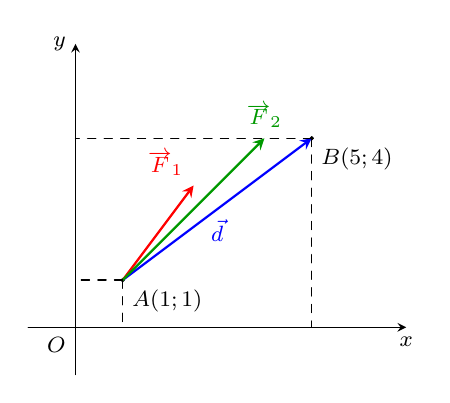
\begin{tikzpicture}[scale=0.6, font=\footnotesize, line join=round, line cap=round, >=stealth]
	\draw[->] (-1,0) -- (7,0) node[below] {$x$};
	\draw[->] (0,-1) -- (0,6) node[left] {$y$};
	\draw (0,0) node[below left] {$O$};
	\coordinate (A) at (1,1);
	\coordinate (B) at (5,4);
	\draw[fill=black] (A) circle (1pt) node[below right] {$A(1;1)$};
	\draw[fill=black] (B) circle (1pt) node[below right] {$B(5;4)$};
	\draw[->, thick, blue] (A) -- (B) node[midway, below] {$\vec{d}$};
	\draw[->, thick, red] (A) -- +(1.5,2) node[above left] {$\overrightarrow{F}_1$};
	\draw[->, thick, green!60!black] (A) -- +(3,3) node[above] {$\overrightarrow{F}_2$};
	\draw[dashed] (1,1) -- (1,0) (5,4) -- (5,0) (1,1) -- (0,1) (5,4) -- (0,4);
	\end{tikzpicture}}
\loigiai{
	Vectơ dịch chuyển $\vec{AB} = (5-1; 4-1) = (4;3)$.\\
	Lực $\overrightarrow{F}_2$ có độ lớn $10\sqrt{2}$ và tạo với $Ox$ góc $45^\circ$ nên
	$$\overrightarrow{F}_2 = (10\sqrt{2} \cdot \cos 45^\circ; 10\sqrt{2} \cdot \sin 45^\circ) = (10;10).$$
	Tổng hợp lực tác động lên vật là
	$$\vec{F} = \overrightarrow{F}_1 + \overrightarrow{F}_2 = (3+10; 4+10) = (13;14).$$
	Tổng công sinh bởi hai lực là
	$$W = \vec{F} \cdot \vec{AB} = 13 \cdot 4 + 14 \cdot 3 = 52 + 42 = 94 \ (\text{J}).$$
	}
\end{ex}
\begin{ex}%[0H5V4-7]%[Biên soạn tài liệu dạy học bộ KNTT - CS]%[GVBS Nguyễn Hữu Chung Kiên]
	Một vật đang ở vị trí $O$ chịu hai lực tác dụng ngược chiều nhau là $\overrightarrow{F}_1$ và $\overrightarrow{F}_2$, trong đó độ lớn lực $\overrightarrow{F}_2$ lớn gấp đôi độ lớn lực $\overrightarrow{F}_1$. Người ta muốn vật dừng lại nên cần tác dụng vào vật hai lực $\overrightarrow{F}_3, \overrightarrow{F}_4$ có phương hợp với lực $\overrightarrow{F}_1$ các góc $45^{\circ}$ như hình vẽ, chúng có độ lớn bằng nhau và bằng $20$ N. Tính tổng độ lớn của các lực $\overrightarrow{F}_1$, $\overrightarrow{F}_2$. (\textit{đơn vị N, kết quả làm tròn đến hàng đơn vị})
	\begin{center}
		\begin{tikzpicture}[scale=.7,>=stealth]
			\coordinate [label=above left:$O$](O) at (0,0);
			\coordinate (A) at (6,0);
			\coordinate (B) at (-12,0);
			\coordinate (C) at  (3,3);
			\coordinate (D) at  (3,-3);	\foreach \diem in {O}	\fill (\diem)circle(1pt);
			\draw[->](O)--(A);
			\draw[->](O)--(B);
			\draw[->, dashed](O)--(C);
			\draw[->, dashed](O)--(D);
			\draw pic[draw, angle radius=4mm]{angle=A--O--C};
			\draw pic[draw, angle radius=6mm]{angle=D--O--A};
			\draw($(O)! .5 ! (B)$)node [above]{$\overrightarrow{F}_2$};
			\draw($(O)! .5 ! (A)$)node [above right]{$\overrightarrow{F}_1$};
			\draw($(O)! .5 ! (C)$)node [above left]{$\overrightarrow{F}_3$};
			\draw($(O)! .5 ! (D)$)node [below left]{$\overrightarrow{F}_4$};
			\draw(1.2,.4)node {$45^\circ$};
			\draw(1.4,-.4)node {$45^\circ$};
			\draw (O) circle (3);
		\end{tikzpicture}
	\end{center}
	\shortans{$85$}
\loigiai{
	Theo giả thiết, $\overrightarrow{F}_1$ và $\overrightarrow{F}_2$ ngược chiều và $\left|\overrightarrow{F}_2\right| = 2\left|\overrightarrow{F}_1\right|$ nên $\overrightarrow{F}_2 = -2\overrightarrow{F}_1$.\\
	Để vật đứng yên (cân bằng) thì tổng hợp lực tác dụng lên vật phải bằng $\vec{0}$
	$$\overrightarrow{F}_1 + \overrightarrow{F}_2 + \overrightarrow{F}_3 + \overrightarrow{F}_4 = \vec{0} \Leftrightarrow \overrightarrow{F}_1 - 2\overrightarrow{F}_1 + \overrightarrow{F}_3 + \overrightarrow{F}_4 = \vec{0} \Leftrightarrow \overrightarrow{F}_1 = \overrightarrow{F}_3 + \overrightarrow{F}_4.$$
	Bình phương vô hướng hai vế đẳng thức trên, ta được
	\allowdisplaybreaks
	\begin{eqnarray*}
		\overrightarrow{F}_1^2 &=& \left(\overrightarrow{F}_3 + \overrightarrow{F}_4\right)^2 \\
		\left|\overrightarrow{F}_1\right|^2 &=& \overrightarrow{F}_3^2 + \overrightarrow{F}_4^2 + 2\overrightarrow{F}_3 \cdot \overrightarrow{F}_4 \\
		\left|\overrightarrow{F}_1\right|^2 &=& \left|\overrightarrow{F}_3\right|^2 + \left|\overrightarrow{F}_4\right|^2 + 2\left|\overrightarrow{F}_3\right| \cdot \left|\overrightarrow{F}_4\right| \cdot \cos\left(\overrightarrow{F}_3, \overrightarrow{F}_4\right).
	\end{eqnarray*}
	Theo hình vẽ, góc giữa $\overrightarrow{F}_3$ và $\overrightarrow{F}_1$ là $45^\circ$ (hướng lên), góc giữa $\overrightarrow{F}_4$ và $\overrightarrow{F}_1$ là $45^\circ$ (hướng xuống). Suy ra góc giữa $\overrightarrow{F}_3$ và $\overrightarrow{F}_4$ là $45^\circ + 45^\circ = 90^\circ$.\\
	Thay số với $\left|\overrightarrow{F}_3\right| = \left|\overrightarrow{F}_4\right| = 20$ và $\cos 90^\circ = 0$
	$$\left|\overrightarrow{F}_1\right|^2 = 20^2 + 20^2 + 2 \cdot 20 \cdot 20 \cdot 0 = 800 \Rightarrow \left|\overrightarrow{F}_1\right| = \sqrt{800} = 20\sqrt{2}\text{ (N)}.$$
	Suy ra $\left|\overrightarrow{F}_2\right| = 2\left|\overrightarrow{F}_1\right| = 40\sqrt{2}$ (N).\\
	Vậy tổng độ lớn hai lực là
	$$\left|\overrightarrow{F}_1\right| + \left|\overrightarrow{F}_2\right| = 20\sqrt{2} + 40\sqrt{2} = 60\sqrt{2} \approx 85 \text{ (N)}.$$
	}
\end{ex}
\Closesolutionfile{ans}
\indapan{3}{ans/0-KNTT-C4B11-kq}
%------------------Tự luận
\ind{PHẦN IV.} \inden{Tự luận.}
\setcounter{ex}{0}
\begin{ex}%[0H9H2-2]%[Biên soạn tài liệu dạy học bộ KNTT - CS]%[GVBS Nguyễn Hữu Chung Kiên]
	Trong mặt phẳng toạ độ $Oxy$, cho tam giác $ABC$, biết $A(2;-2)$, $B(3;-4)$, $C(0;-8)$. Tính góc $A$ của tam giác $ABC$.
\loigiai{
	Ta có $\widehat{BAC}=\left(\overrightarrow{AB},\overrightarrow{AC}\right)$,
	$\overrightarrow{AB}=(1;-2)$, $\overrightarrow{AC}=(-2;-6)$.\\
	$\Rightarrow \cos\left(\overrightarrow{AB},\overrightarrow{AC}\right)=\dfrac{\overrightarrow{AB}.\overrightarrow{AC}}{\left|\overrightarrow{AB}\right|\cdot \left|\overrightarrow{AC}\right|}=\dfrac{1\cdot (-2)+(-2)\cdot (-6)}{\sqrt{1^2+(-2)^2}\cdot \sqrt{(-2)^2+(-6)^2}}=\dfrac{\sqrt{2}}{2}$.\\
	$\Rightarrow \widehat{BAC}=\left(\overrightarrow{AB},\overrightarrow{AC}\right)=45^\circ$.
	}
\end{ex}
\begin{ex}%[0H5H4-1] %[Biên soạn tài liệu dạy học bộ KNTT - CS]%[GVBS Nguyễn Hữu Chung Kiên]
	Cho hình bình hành $ABCD$, với $AB=2$, $AD=1$, $\widehat{BAD}=60^\circ $. Tính tích vô hướng $\overrightarrow{AB}\cdot \overrightarrow{AD}$.
\loigiai{
	$\overrightarrow{AB}\cdot \overrightarrow{AD}=\left| \overrightarrow{AB} \right|\cdot \left| \overrightarrow{AD} \right|\cdot \cos \left( \overrightarrow{AB},\overrightarrow{AD} \right)=AB\cdot AD\cdot \cos \widehat{BAD}=2\cdot 1\cdot \cos 60^{\circ}=1$.}
\end{ex}
\begin{ex}%[0H5H4-7]%[Biên soạn tài liệu dạy học bộ KNTT - CS]%[GVBS Nguyễn Hữu Chung Kiên]
	Một người dùng một lực kéo $\overrightarrow{F}$ có độ lớn $40$ N để kéo một thùng gỗ trượt trên sàn nhà một khoảng cách $20$ m. Biết rằng góc hợp bởi vectơ lực $\overrightarrow{F}$ và hướng chuyển động của thùng gỗ là $60^{\circ}$. Tính công sinh bởi lực $\overrightarrow{F}$.
	\loigiai
	{Gọi $\overrightarrow{d}$ là vectơ độ dịch chuyển của thùng gỗ.\\
	Theo đề bài, ta có $\left|\overrightarrow{F}\right| = 40\,\mathrm{N}$, $\left|\overrightarrow{d}\right| = 20$ m và góc giữa hai vectơ $\left( \overrightarrow{F}, \overrightarrow{d} \right) = 60^{\circ}$.\\
	Công sinh bởi lực $\overrightarrow{F}$ được tính theo công thức tích vô hướng
	$$A = \overrightarrow{F} \cdot \overrightarrow{d} = \left|\overrightarrow{F}\right| \cdot \left|\overrightarrow{d}\right| \cdot \cos \left( \overrightarrow{F}, \overrightarrow{d} \right)= 40 \cdot 20 \cdot \cos 60^{\circ} = 800 \cdot \dfrac{1}{2} = 400.$$
	Vậy công sinh bởi lực $\overrightarrow{F}$ là $400$ J.}
\end{ex}
\begin{ex}%[0H9V2-7]%[Biên soạn tài liệu dạy học bộ KNTT - CS]%[GVBS Nguyễn Hữu Chung Kiên]
	Trong mặt phẳng tọa độ $Oxy$ với đơn vị đo trên các trục là mét, một robot thông minh di chuyển thẳng từ vị trí $A(5; 2)$ đến vị trí $B(9; 5)$. Trong quá trình di chuyển, robot chịu tác động của một lực kéo không đổi $\overrightarrow{F}$ có tọa độ là $\overrightarrow{F} = (20; 10)$ (đơn vị N). Tính công sinh bởi lực $\overrightarrow{F}$.
	\loigiai
	{Vectơ độ dịch chuyển của robot là $\overrightarrow{d} = \overrightarrow{AB}$.\\
	Ta có $\overrightarrow{AB} = (9 - 5; 5 - 2) = (4; 3)$.\\
	Công sinh bởi lực $\overrightarrow{F}$ được tính bằng tích vô hướng của vectơ lực $\overrightarrow{F}$ và vectơ độ dịch chuyển $\overrightarrow{d}$.
	$$A = \overrightarrow{F} \cdot \overrightarrow{d} = 20 \cdot 4 + 10 \cdot 3 = 80 + 30 = 110.$$
	Vậy công sinh bởi lực $\overrightarrow{F}$ là $110$ J.}
\end{ex}
\begin{ex}%[0H5V4-7]%[Biên soạn tài liệu dạy học bộ KNTT - CS]%[GVBS Nguyễn Hữu Chung Kiên]
	Hai con tàu kéo cùng tác dụng lực lên một chiếc sà lan đang mắc kẹt. Tàu thứ nhất kéo với lực $\overrightarrow{F}_1$ có độ lớn $300$ N, tàu thứ hai kéo với lực $\overrightarrow{F}_2$ có độ lớn $500$ N. Biết rằng dây cáp của hai tàu hợp với nhau một góc $60^{\circ}$. Tính độ lớn của hợp lực $\overrightarrow{F} = \overrightarrow{F}_1 + \overrightarrow{F}_2$ tác dụng lên sà lan.
	\loigiai
	{Ta cần tính độ lớn của vectơ hợp lực $\overrightarrow{F} = \overrightarrow{F}_1 + \overrightarrow{F}_2$.\\
	Bình phương vô hướng hai vế, ta được
	$$ \overrightarrow{F}^2 = \left( \overrightarrow{F}_1 + \overrightarrow{F}_2 \right)^2 = \overrightarrow{F}_1^2 + \overrightarrow{F}_2^2 + 2\overrightarrow{F}_1 \cdot \overrightarrow{F}_2. $$
	Áp dụng công thức tích vô hướng $\overrightarrow{F}_1 \cdot \overrightarrow{F}_2 = \left|\overrightarrow{F}_1\right| \cdot \left|\overrightarrow{F}_2\right| \cdot \cos 60^{\circ}$, ta có
	$$ \begin{aligned} |\overrightarrow{F}|^2 &= 300^2 + 500^2 + 2 \cdot 300 \cdot 500 \cdot \cos 60^{\circ} \\ &= 90\,000 + 250\,000 + 300\,000 \cdot \dfrac{1}{2} \\ &= 340\,000 + 150\,000 \\ &= 490\,000. \end{aligned} $$
	Suy ra độ lớn hợp lực là $\left|\overrightarrow{F}\right| = \sqrt{490\,000} = 700$ N.\\
	Vậy độ lớn của hợp lực là $700$ N.}
\end{ex}
\begin{ex}%[0H9V2-7]%[Biên soạn tài liệu dạy học bộ KNTT - CS]%[GVBS Nguyễn Hữu Chung Kiên]
	Trong mặt phẳng tọa độ $Oxy$ (đơn vị trên các trục là mét), một hành lang thẳng được biểu diễn bởi trục hoành $Ox$. Có hai camera giám sát được đặt cố định tại vị trí $A(10; 20)$ và $B(60; 30)$. Một bảo vệ đi tuần tra dọc theo hành lang này. Biết rằng có đúng hai vị trí trên hành lang mà tại đó góc nhìn từ người bảo vệ đến hai camera là $90^{\circ}$. Tính khoảng cách giữa hai vị trí đó theo đơn vị m.
	\loigiai
	{Gọi vị trí của người bảo vệ trên hành lang là điểm $M$. Vì $M$ nằm trên trục hoành $Ox$ nên tọa độ của $M$ có tọa độ $M(x; 0)$.\\
	Ta có tọa độ các vectơ
	$$ \overrightarrow{MA} = (10 - x; 20); \quad \overrightarrow{MB} = (60 - x; 30). $$
	Góc nhìn từ người bảo vệ đến hai camera là $\widehat{AMB} = 90^{\circ}$, suy ra $\overrightarrow{MA} \perp \overrightarrow{MB}$, hay tích vô hướng $\overrightarrow{MA} \cdot \overrightarrow{MB} = 0$.\\
	Khi đó ta có phương trình
	\begin{align*}
		&\overrightarrow{MA} \cdot \overrightarrow{MB} = 0\\
		\Leftrightarrow\ & (10 - x)(60 - x) + 20 \cdot 30 = 0 \\
		\Leftrightarrow \ & 600 - 10x - 60x + x^2 + 600 = 0 \\
		\Leftrightarrow \ & x^2 - 70x + 1\,200 = 0\\
		\Leftrightarrow \ & x_1 = 30 \vee x_2 = 40.
	\end{align*}
	Như vậy, hai vị trí thỏa mãn đề bài là $M_1(30; 0)$ và $M_2(40; 0)$.\\
	Khoảng cách giữa hai vị trí này là
	$$ M_1M_2 = |x_2 - x_1| = |40 - 30| = 10.$$
	Vậy khoảng cách cần tìm là $10$ m.}
\end{ex}
\Closesolutionfile{ans}
%\end{document}